\documentclass{article}
\usepackage[utf8]{inputenc}
\usepackage[T1]{fontenc}
\usepackage{tgtermes}
\usepackage{mathptmx}  
\usepackage[scaled=.92]{helvet}
\usepackage{amsthm,amsmath,amssymb}
\usepackage{mathrsfs}
\usepackage[round]{natbib}  
\usepackage[colorlinks,citecolor=blue,urlcolor=blue]{hyperref}  %%check
\usepackage[dvipsnames]{xcolor}
%%%Algorithms
\usepackage[noend]{algpseudocode}
\usepackage{algorithm,amsmath}
\usepackage{mathtools}
\usepackage{newtxtext,newtxmath}
\usepackage[tight,footnotesize]{subfigure}
\usepackage[colorinlistoftodos]{todonotes}
\newcommand*{\R}{\mathbb{R}}
\newcommand*{\G}{\mathcal{G}}
\newcommand*{\Po}{\text{Prox}}
\newcommand*{\Am}{\text{argmin}}
\newcommand*{\E}{\mathbb{E}}
\newcommand*{\VRG}{\,\tilde{\nabla}_k^s}
\newcommand{\norm}[1]{\left\lVert#1\right\rVert}
\newcommand{\abs}[1]{\left|#1\right|}
\newcommand{\Iprod}[2]{\left\langle #1,#2\right\rangle}
\newcommand\myeq[2]{\mathrel{\stackrel{\makebox[0pt]{\mbox{#1}}}{#2}}}

\renewcommand{\algorithmicrequire}{
\textbf{Input:}}
\renewcommand{\algorithmicensure}{\textbf{Output:}}
\newcommand{\Initialize}{\textbf{Initialize:}{\,}}
\newcommand{\Input}{\textbf{Input:}{\,}}
\newcommand{\Output}{\textbf{Output:}{\,}}


\newtheorem{theorem}{Theorem}[section]
\newtheorem{lemma}[theorem]{Lemma}
\newtheorem{conjecture}[theorem]{Conjecture}
\newtheorem{condition}[theorem]{Condition}
\newtheorem{claim}[theorem]{Claim}
\newtheorem{question}[theorem]{Question}
\newtheorem{corollary}[theorem]{Corollary} 
\theoremstyle{definition}
\newtheorem{definition}[theorem]{Definition}
\newtheorem{statement}[theorem]{Statement}
\newtheorem{notation}[theorem]{Notation} 
\theoremstyle{remark}
\newtheorem{remark}[theorem]{Remark}
\newtheorem{assumption}[theorem]{Assumption}
\allowdisplaybreaks

\title{An Acceleration of Derivative-Free Proximal Stochastic Gradient Method for Nonconvex Nonsmooth Optimization}
\date{March 2018}

\begin{document}

\maketitle
\begin{abstract}
We provide a simpler analysis with better dependence on dimension of problem $d$. 
\end{abstract}

\section{Introduction}
\subsection{what we want to do}
{\color{Green}\label{problem}
{\color{Violet}
In this paper, we consider nonsmooth nonconvex finite-sum optimization problems of the form
}
\begin{equation}
\min_{x\in\R^d} F(x) =  f(x) + h(x),\,\,\,f(x):=\frac{1}{n}\sum_{i=1}^n f_i(x)
\end{equation}
where each $f_i(x)$ is {\color{Violet} possibly} nonconvex and smooth loss function, and $h(x)$ is a nonsmooth but convex structure regularizer such as $l_1$-norm regularization. }
{\color{Brown}
The generic form \eqref{problem} encompasses
many machine learning problems, ranging from generalized linear models to neural networks 
{\color{Violet} and from convex optimization such as Lasso, SVM to highly nonconvex problem such as optimizing deep neural networks.}


We will study and analysis of {\color{Green} a class of} variance reduced and faster converging stochastic zeroth-order (SZO) optimization methods for \eqref{problem}. The stochastic variance reduced gradient
(SVRG) is a commonly-used, effective first-order approach to reduce the variance \cite{johnson2013accelerating,reddi2016stochastic,nitanda2016accelerated,allen2016improved,lei2017non}. Due to
the variance
reduction, it improves the convergence rate of stochastic gradient descent (SGD) complexity from
$O(1/\epsilon^2)$ to $O(1/{\epsilon})$. To reduce the variance accelerate SZO optimization, one can draw
motivations from similar ideas in the first-order regime. 


}

\subsection{Background in research}
{\color{Green}
In recent research \cite{beck2009fast},
the accelerated proximal gradient (PG) methods are proposed to solve convex problems by using the Nesterov's accelerated technique.  
}
{\color{Violet}
After that, there has been extensive research when $f(x)$ is convex (see e.g., {  
\cite{nesterov2013gradient}}, \cite{xiao2014proximal,defazio2014saga,lan2017optimal,allen2017katyusha}. In particular, if each $f_i$ is strongly-convex, \cite{xiao2014proximal} proposed the Prox-SVRG algorithm {\color{green} for large-scale problems}, which achieves a linear convergence rate, based on the well-known variance reduction technique SVRG
developed in \cite{johnson2013accelerating}. To solve the big data problems, the incremental or stochastic PG methods \cite{bertsekas2011incremental,xiao2014proximal} were developed for large-scale convex optimization. In recent years, due to the increasing popularity of deep learning, the nonconvex case has attracted significant attention. For a general nonsmooth nonconvex case, the research is still somewhat limited.  \cite{li2015accelerated} presented a class of accelerated PG methods for nonconvex optimization. {\color{Green} Correspondingly, \cite{ghadimi2016accelerated,reddi2016proximal} proposed the stochastic PG methods for large-scale nonconvex optimization.}
Very recently, \cite{li2018simple} proposed an algorithm generalized the results by \cite{reddi2016proximal} and improved the stochastic gradient complexity. 
}
\subsection{Reason to use zeroth--order techniques}

{\color{DarkOrchid}
The main issue for these accelerated algorithms is that most of their algorithm designs involve computing first-order information. 
}
{\color{Green}
{\color{RubineRed}
However, there exist situations where the first-order gradient information is computationally infeasible, expensive, or impossible,
while the zeroth-order functional information can be easily obtained
}

{\color{RubineRed}
 For example, in online auctions and advertisement
selections, only function values are revealed as feedbacks for algorithms \cite{wibisono2012finite}. In stochastic structured predictions, explicit differentiations may be difficult to perform while the functional evaluations of predicted structures are easily obtained \cite{sokolov2016stochastic}. }

For example, in bandit \cite{shamir2017optimal} and black-box learning \cite{chen2017zoo} problems, only the objective function values are available (the explicit gradients cannot be calculated). 
The gradient-free  optimization method \cite{nesterov2017random} is a promising choice to address these problems because it only uses the function values in optimization process. {\color{Brown} These algorithms achieve gradient-free optimization by approximating the full gradient via gradient estimators based on only the function values \cite{brent2013algorithms,spall2005introduction}.} 
{\color{RubineRed} We refer the optimization problem of equation \eqref{problem} in such situations as stochastic proximal zeroth-order optimization.}
{\color{YellowOrange}
Zeroth-order optimization has recently gained increasing
attention due to its wide usage in many applications where
the explicit expressions of gradients of the objective function are expensive or infeasible to obtain and only function
evaluations are accessible. Such a class of applications include black-box adversarial attacks on deep neural networks
(DNNs) (Papernot et al., 2017; Chen et al., 2017; Kurakin
et al., 2016), structured prediction (Taskar et al., 2005) and
reinforcement learning (Choromanski et al., 2018).
}
}
{\color{Brown}
Additional classes of applications include network control and management with time-varying constraints and limited computation capacity \cite{chen2019bandit,liu2017zeroth}, and parameter inference of black-box systems \cite{fu2002optimization,lian2016comprehensive}. 
}

{\color{DarkOrchid}
The main issue for those accelerated algorithms is that most of their algorithm designs (e.g., (Allen-Zhu, 2017)
and (Hien et al., 2017)) involve tracking at least two highly
correlated coupling vectors 2 (in the inner loop). This kind
of algorithm structure prevents us from deriving efficient
(lock-free) asynchronous sparse variants for those algorithms.
}
\subsection{Problem with existing methods}
{\color{Brown}
Although many SZO algorithms have recently been developed and analyzed \cite{liu2017zeroth,flaxman2005online,shamir2013complexity,agarwal2010optimal,nesterov2017random,duchi2015optimal,shamir2017optimal,dvurechensky2018accelerated,wang2017stochastic}, they are mainly designed for convex settings, which limits their applicability in a wide range of (nonconvex) machine learning problems.

 In addition, these algorithms often suffer from the high variances of SZO gradient estimates, and in turn, hampered convergence rates. {\color{RubineRed}
Thus, a useful technique to accelerate the convergence of SZO is by leveraging variance reduction method.
}
}
{\color{YellowOrange}
Recently, several zeroth-order stochastic variance
reduced algorithms have been developed to further improve
the convergence rate of ZO-SGD \cite{liu2018stochastic,liu2018zeroth}. These algorithms are mainly based on SVRG algorithm, which replaces the gradient in
SVRG \cite{johnson2013accelerating} by zeroth-order gradient
estimators. In particular, \cite{liu2018zeroth} proposed three
zeroth-order SVRG-based algorithms. 

} 
{\color{Green}  Until now, there are few zeroth-order stochastic methods
for solving the problem \eqref{problem} e.g., \cite{ghadimi2016accelerated} and \cite{huang2019faster}. Specifically, \cite{ghadimi2016accelerated} have proposed a randomized stochastic projected gradient-free method (RSPGF),
i.e., a zeroth-order proximal stochastic gradient method. However, due to the large variance of zeroth-order estimated gradient generated from randomly selecting the sample and the direction of derivative, RSPGE only has a iteration complexity of  $O(\frac{d}{\epsilon^2})$ based on two function evaluations, which is significantly slower than $O(\frac{d}{{\epsilon}})$,
the best known convergence rate of the zeroth-order stochastic algorithm. 
{\color{RubineRed}
A key concern in the development of iterative stochastic zeroth-oder algorithms for solving  \eqref{problem} is the order of the necessary number of functional evaluations, namely SZO calls or iteration complexity.
}
{\color{YellowOrange}
Although the existing zeroth-order SVRG-based algorithms have improved iteration rate of convergence
, their function query complexities are all larger than either ZO-GD or ZO-SGD. They also require a very small stepsize of $O(\frac{1}{d})$.  \cite{ji2019improved} improved the analysis to obtain better ZO complexity and convergence rate. However the parameters in their analysis are very involved and the improvement is based on a very large minibatch sizes.
}
{\color{Brown}
 Without a
careful treatment, the dimension dependent factor in the convergence rate (i.e., $d$) could be a critical factor affecting
the optimization performance. To mitigate this factor, we propose an accelerated ZO proximal  variants, utilizing reduced variance gradient estimators for nonsmooth composite optimization. These yield a faster iteration complexity towards $O(1/\epsilon )$, which is, to our knowledge, the best iteration complexity bound so far achieved for proximal ZO stochastic optimization with nonconvex structure.
{\color{RubineRed} This indicates an improvement over existing results up to a factor of ${d}$.}

}
}

\subsection{Compare with other methods}
{\color{Violet}
We list the results of proposed algorithms and other related ones in Table \ref{table-compare}.
}
{\color{Brown}

Table \ref{table-compare} shows
that RGF has the highest query complexity and nevertheless has the worst convergence rate. ZO-SVRG-coord
and ZO-ProxSVRG/SAGA yield the best convergence rate in the cost of high query complexity. {\color{YellowOrange} However, existing SVRG type zeroth-order algorithms suffer from worse
function query complexities than stochastic proximal gradient descent (RSPGF).} By contrast, ZO-PSVRG+ could achieve better trade-offs between the
convergence rate and the query complexity.
}



\section{Main Challenge}
{\color{Brown}
Although proximal SVRG has shown a great promise, applying similar ideas to ZO optimization is not a trivial
task. 
{\color{DarkOrchid}
Zeroth-order method are applicable for problem that the first-order gradient is not available, but, due to the existence of
perturbation, gradient estimation has complex coupling structures, which makes
them hard to be extended to more settings. 
}
The other main challenge is due to the fact that ProxSVRG relies upon the assumption that a stochastic gradient is an unbiased estimate of the true batch/full gradient, which unfortunately does not hold in the ZO case. Therefore, it is an open question whether the proximal ZO stochastic variance reduced gradient could enable faster convergence of ZO algorithms. In this paper, we attempt to fill the gap between
SZO optimization and ProxSVRG and improve the efficiency of exiting ZO variance reduced methods for problem \eqref{problem}.
}


\section{Main contributions}

{\color{Green}

{\color{YellowOrange}
We develop a new analysis for an existing ZO-SVRG-Coord algorithm proposed in \cite{liu2018zeroth,ji2019improved}, and
show that ZO-PSVRG+ (under our new analysis) outperforms other exiting SVRG-type zeroth-order methods as well as RSPGF.
} 
{\color{Brown}
We addresses several important issues that are still open in these methods. In particular, we partially answer the open question if the dependence on the dimension $d$ for the convergence analysis proposed in \cite{liu2018zeroth} is optimal. Our work offers a comprehensive study on how ZO gradient estimators affect ProxSVRG on both iteration complexity (i.e., convergence rate) and function query complexity. This
is accomplished by a novel synthesis of existing SZO algorithms.

 
} 
{\color{Violet}
The main technical contribution lies in the new convergence analysis of ZO-PSVRG+,
which has notable difference from that of ZO-SVRG \cite{liu2018zeroth}, ZO-ProxSVRG \cite{huang2019faster} and ZO-SVRG-Coord-Rand \cite{ji2019improved}. {\color{Brown} Note that our considered problem does not necessarily satisfy bounded gradients assumption in \cite{ghadimi2016accelerated,huang2019faster}.}
We show that compared to
ProxSVRG, ZO-PSVRG+ achieves a similar convergence with SZO complexity of $O(1/\epsilon)$.
The convergence results are stated in terms of the number of stochastic zeroth-order (SZO) calls and proximal oracle (PO) calls. 
} 
 

{\color{Violet}
We would like to highlight the following results yielded by our new analysis:

1) Our analysis provides iteration complexity $O(\frac{1}{{\epsilon}})$ compared with $O(\frac{d}{\epsilon^2})$ of RSPGF \cite{ghadimi2016accelerated}  and $O(\frac{d}{\epsilon})$ of ZO-ProxSVRG/SAGA  \cite{huang2019faster} (the existing variance-reduce SZO proximal algorithm for solving nonconvex nonsmooth problems).  
{\color{RubineRed}In other words, the proposal expectational results have better or no dependence on
$d$ compared to the existing variance-reduced SZO methods.} Note that the number of PO calls equal to $O(1/\epsilon)$  and $O(1/\epsilon^2)$ for ZO-PSVRG+ and RSPGF, respectively.  ZO-PSVRG+ also matches the best result achieved by ZO-SVRG-Coord-Rand with $b = d n^{2/3}$ for $m = n^{1/3}$ in \cite{ji2019improved}. Note that our rate of convergence is valid for any minibatch sizes as detailed in the following sections.  
} In fact, since practitioners typically use moderate minibatch sizes, it is important to study and show the convergence in moderate and constant minibatch size regime.


{\color{Violet} 2) ZO-PSVRG+ is more straightforward than ZO-SVRG-Coord proposed and analyzed by \cite{liu2018zeroth,ji2019improved} very recently, and yields simpler proof.  
}{\color{YellowOrange}
Our analysis develops new complexity bounds and order-wisely improves the performance of not only all existing zeroth-order SVRG-based algorithms
(see Table \ref{}) but also RSPGF for nonconvex nonsmooth composite optimization, which is the first time to the best of our knowledge. 
}



}
{\color{Violet}
3) For the nonconvex functions satisfying Polyak-Łojasiewicz condition \cite{polyak1963gradient}, we prove that ZO-PSVRG+
achieves a global linear convergence rate similar to first-order ProxSVRG. Thus, ZO-PSVRG+ can automatically switch to
the faster linear convergence in some regions without restart and algorithmic modification. To the best of
our knowledge, this is the first paper that leverages the PL condition for improving the convergence of of ZO-ProxSVRG for problem \eqref{problem} with arbitrary minibatch size. It is also notable that the convergence rate achieved in this case can be as good as first-order ProxSVRG. This generalizes the results of MD \cite{duchi2015optimal} and  achieves linear convergence compared with sublinear rate of MD, (see Table \ref{table-compare}).
It is shown in \cite{ji2019improved} that  ZO-SPIDER-Coord under PL condition achieves linear condition with $b = O(n^{1/2})$.  
{\color{Violet} Note that from the perspectives of both computational and statistical efficiency, reasonable minibatch size is desirable in practice, since the computation of minibatch stochastic gradients can be
implemented in parallel. 
} Also see the remarks after Theorem \ref{zo-pl-cond} for more details. {\color{RubineRed}

}
}


{\color{Brown}
 Finally, to demonstrate the flexibility of our approach in managing trade-off between the rate of convergence and the number of SZO calls, we conduct an
empirical evaluation of our proposed algorithms and other state-of-the-art algorithms on two diverse
applications: black-box chemical material classification and generation of universal adversarial
perturbations from black-box deep neural network models. Extensive experimental results and
theoretical analysis validate the effectiveness of our approaches.
}


\section{Related Works}
{\color{Green}
Gradient-free (zeroth-order) methods have been effectively used to solve many machine learning problems, where the explicit gradient is difficult or infeasible to obtain, and have also been widely studied. 
{\color{Brown}
In ZO algorithms, a full gradient is typically approximated using either a one-point or a two-point gradient estimator, where the former acquires a gradient estimate $\hat{\nabla} f(x)$ by querying $f$ at a single random location close to $x$ \cite{flaxman2005online,shamir2013complexity}, and the latter computes a finite difference using two random function queries \cite{agarwal2010optimal,nesterov2017random}. In this paper, we focus on the two-point gradient estimator since it has a lower variance and thus improves the complexity bounds of ZO algorithms.
}

\cite{nesterov2017random} proposed several random gradient-free
methods by using Gaussian smoothing technique. \cite{duchi2015optimal} proposed a zeroth-order mirror descent algorithm. 

{\color{Brown}

 More recently, \cite{yu2018generic,dvurechensky2018accelerated} presented the accelerated zeroth-order methods for the convex optimization. Current studies suggested that ZO algorithms typically agree with the iteration complexity of first-order
algorithms up to a small-degree polynomial of the problem size $d$.

{\color{Green} The above zeroth-order methods mainly focus on the
(strongly) convex problems. Thus, exploring zeroth-order stochastic methods for the nonconvex optimization is indeed desirable. In fact, there exist many nonconvex machine learning tasks, whose explicit gradients are not available, such as the nonconvex black-box learning problems \cite{chen2017zoo,liu2018zeroth}. 
{\color{Brown}
In contrast to the convex setting, nonconvex ZO algorithms are comparatively under-studied.
}
{\color{YellowOrange}
\cite{ghadimi2013stochastic} and \cite{nesterov2011random} proposed ZO-GD and
its stochastic counterpart ZO-SGD, respectively. \cite{liu2018stochastic} proposed a stochastic
zeroth-order method with variance reduction under Gaussian smoothing. More recently, \cite{liu2018zeroth} provided a comprehensive analysis on SVRG-based algorithms. \cite{ji2019improved} improved the analysis in \cite{liu2018zeroth} and obtained tighter bounds using an involved parameter selection, however their improvements requires very large minibatch sizes. 
}

{\color{Violet}
Recently, for the nonsmooth nonconvex case, \cite{huang2019faster} provided two algorithms called ZO-ProxSVRG and ZO-ProxSAGA, which are based on the well-known variance reduction techniques ProxSVRG and ProxSAGA \cite{reddi2016proximal}. Before that,  \cite{ghadimi2016accelerated} also considered the stochastic case (here we denote
it as RSPGF). However, RSPGF requires the batch sizes being a large number (i.e., $\Omega(1/\epsilon)$) or increasing with
iterations. Note that RSPGF may reduce to deterministic proximal gradient descent (ZO-ProxGD) after some iterations due to the
increasing batch sizes.
}
Moreover, to solve the large-scale machine learning problems, some asynchronous parallel stochastic zeroth-order algorithms have been proposed in \cite{gu2018inexact,lian2016comprehensive,gu2018faster}.
}
In \cite{lian2016comprehensive}, an asynchronous ZO stochastic coordinate
descent (ZO-SCD) was derived for parallel optimization and achieved the rate of $O(d/\epsilon^2)$.
{\color{YellowOrange} \cite{gu2018faster} further improved the convergence rate of
asynchronous SZO by combining SVRG technique with coordinate-wise gradient. }
{\color{Violet} Note that from the perspectives of both computational efficiency and statistical generalization, always computing full-gradient may not be desirable for large-scale machine learning problems.} This motivates our study on a more general framework ZO-SVRG under different gradient estimators.
}

\subsection{Motivation at the end of related works}
Although the above zeroth-order stochastic methods can effectively solve the nonconvex optimization, there are few zeroth-order stochastic methods for the nonconvex nonsmooth composite optimization except the RSPGF method presented in \cite{ghadimi2016accelerated} and ZO-ProxSVRG/SAGA \cite{huang2019faster}. We emphasize that, unlike these methods, we do not assume  bounded gradient since it is not the case for many unconstrained optimization problems. In addition, \cite{liu2018stochastic} have also studied the zeroth-order algorithm for solving the nonconvex nonsmooth problem, which is different from problem \eqref{problem}.
}
\begin{table}\label{table-compare}
\begin{center}
\begin{tabular}{ |l|l|l|l|l| } 
 \hline
 Method & Problem & Stepsize& Convergence rate & SZO complexity\\ 
 \hline
  
 RGF\cite{nesterov2017random} & NS(C) & $O\left(\frac{1}{\sqrt{dT}}\right)$ & $O\left(\frac{d^2}{\epsilon^2}\right)$ &$O\left(\frac{nd^2}{\epsilon^2}b\right)$\\
 RSPGF\cite{ghadimi2016accelerated} & S(NC)+NS(C) & $O\left(1\right)$ & $O\left(\frac{d}{\epsilon^2}\right)$ &$O\left(\frac{nd}{\epsilon^2}\right)$\\ 
 ZO-SVRG-Coord \cite{liu2018zeroth} & S(NC)& $O\left(\frac{1}{{d}}\right)$ & $O\left(\frac{d}{\epsilon}\right)$ & $O(\frac{nd^2}{\epsilon}+\frac{d^2b}{\epsilon})$\\
 ZO-SVRG-Coord-Rand \cite{ji2019improved} & S(NC)& $O\left(\frac{1}{{dn^{2/3}}}\right)$ & $O\left(\frac{dn^{2/3}}{\epsilon}\right)$ & $O(\min\{\frac{dn^{2/3}}{\epsilon},\frac{d}{\epsilon^{5/3}}\})$\\
  ZO-ProxSVRG-Coord\cite{gu2018faster} & S(NC)+NS(C) & $O\left(\frac{1}{{d}}\right)$ & $O\left(\frac{d}{\epsilon}\right)$ & $O(\frac{nd^2}{\epsilon\sqrt{b}}+\frac{md^2\sqrt{b}}{\epsilon})$\\
   ZO-ProxSAGA-Coord\cite{gu2018faster} & S(NC)+NS(C)& $O\left(\frac{1}{{d}}\right)$ & $O\left(\frac{d}{\epsilon}\right)$ & $O(\frac{nd^2}{\epsilon\sqrt{b}})$\\
   ZO-PSVRG+ (CoordSGE) (Ours)  & S(NC)+NS(C) & $O\left(1\right)$ & $O\left(\frac{1}{\epsilon}\right)$ & $O\left(s_n\frac{d}{\epsilon \sqrt{b}}+\frac{bd}{\epsilon}\right)$\\
   ZO-PSVRG+ (RandSGE) (Ours)  & S(NC)+NS(C) & $O\left(\frac{1}{\sqrt{d}}\right)$ & $O\left(\frac{\sqrt{d}}{\epsilon}\right)$ & $O\left(s_n\frac{d\sqrt{d}}{\epsilon \sqrt{b}}+\frac{b\sqrt{d}}{\epsilon}\right)$\\
   ZO-PSVRG+ (CoordSGE) (Ours) & S(PL)+NS(C) & $O\left(1\right)$ & $O\left(\log(\frac{1}{\epsilon})\right)$ & {\scriptsize$O(s_n \frac{d}{\lambda\sqrt{\gamma} m}\log\frac{1}{\epsilon}+\frac{bd}{\lambda\sqrt{\gamma}}\log\frac{1}{\epsilon})$}\\
   ZO-PSVRG+ (RandSGE) (Ours) & S(PL)+NS(C) & $O\left(\frac{1}{\sqrt{d}}\right)$ & $O\left(\sqrt{d}\log(\frac{1}{\epsilon})\right)$ & {\scriptsize$O(s_n\frac{d\sqrt{d}}{\lambda\sqrt{\gamma} m}\log\frac{1}{\epsilon}+\frac{b\sqrt{d}}{\lambda\sqrt{\gamma}}\log\frac{1}{\epsilon})$}\\
 \hline
\end{tabular}\caption{Summary of convergence rate and function query complexity of SZO algorithms. S: Smooth, NS: Nonsmooth, NC: Nonconvex, C: Convex, SC: Strong Convexity, and PL: Polyak-Łojasiewicz Condition. $s_n = \min\{n, \frac{1}{\epsilon}\}$}.
\end{center}
\end{table}

\subsection{Zeroth-order (ZO) gradient estimators}

{\color{Brown}
We
next provide a background on ZO gradient estimators.
Given an individual cost function $f_i$, a two-point random stochastic gradient estimator (RandSGE) $\hat{\nabla}_r f_i(x)$ is defined \cite{nesterov2017random,gao2018information}
\begin{equation}\label{gradestrand}
\hat{\nabla}_r f_i(x, u_i) = \frac{d(f_i(x+\mu u_i) - f_i(x))}{\mu}u_i,\qquad i\in [n],
\end{equation}
where recall that $d$ is the number of optimization variables, $\mu > 0$ is a smoothing parameter, and
$\{u_i\}$ are i.i.d. random directions drawn from a uniform distribution over a unit sphere \cite{flaxman2005online,shamir2017optimal,gao2018information}. In general, RandSGE is a biased approximation to the true gradient $\nabla f_i(x)$, and its bias reduces as $\mu$ approaches zero. However, in a practical system, if $\mu$ is too small, then the function difference
could be dominated by the system noise and fails to represent the function differential \cite{lian2016comprehensive}.}

{\color{Green}
To obtain a better estimated gradient, we
can use the coordinate gradient estimator
(CoordSGE) \cite{gu2018inexact,gu2018faster,liu2018zeroth} to estimate the gradients as follows:
\begin{equation}\label{gradestcoord}
\hat{\nabla} f_i(x) = \sum_{j=1}^d \frac{f_i(x+\mu_je_j) - f_i(x-\mu_je_j)}{2\mu_j}e_j,\qquad i\in [n],
\end{equation}
where $\mu_j$ is a coordinate-wise smoothing parameter, and $e_j$ is a standard basis vector with $1$ at its $j$-th coordinate,
and $0$ otherwise. 
}
{\color{Brown}
Compared to RandSGE, CoordSGE is deterministic and requires $d$ times more function queries. 
However, {\color{YellowOrange}
our analysis reveals that for zero-order variance-reduced
algorithms, although the coordinate-wise gradient estimator
requires more queries than the two-point gradient estimator,
it guarantees much higher estimation accuracy, which leads
to a larger stepsize and a faster convergence rate}. More details on ZO gradient estimation can be found in \cite{kazemi2018proximal}.
}


\subsection{Accelerated Proximal Gradient Method}
{\color{Green}
Because proximal gradient method needs to compute
the gradient at each iteration, it cannot be applied to solve the problems, where the explicit gradient of function $f(x)$ is
not available. For example, in the black-box machine learning model, only function values (e.g., prediction results) are
available \cite{chen2017zoo}. To avoid computing explicit gradient, we use the zeroth-order gradient estimators \cite{nesterov2017random,liu2018zeroth} to estimate the
gradient only by function values.
Based on the estimated gradients \eqref{gradestcoord}, we give a zeroth-order proximal gradient descent method, which performs  iterations similar to:
\begin{equation}
x_{t}^s= \Po_{\eta h}(x_{t-1}^s - \eta \hat{\nabla} f(x_{t-1}^s)),\qquad t=1, 2, \ldots
\end{equation}
where $\hat{\nabla} f=\frac{1}{n}\sum_{i=1}^n \hat{\nabla} f_i(x)$ and 
\begin{equation}\label{po-operator}
\Po_{\eta h}(x) := \text{arg}\,\,\min_{y\in\R^d}\left(h(y)+\frac{1}{2\eta}\norm{y-x}^2\right)
\end{equation}
}
{\color{Green}


{\color{Violet}
We also assume that the
nonsmooth convex function $h(x)$ in \eqref{problem} is well structured, i.e., the proximal operator \eqref{po-operator} on $h$ can be computed efficiently.

}
}
\section{Accelerated Proximal Gradient Method}


\begin{algorithm}\label{APGnonconvex-Algo}
\caption{ZO-PSVRG+}
\begin{algorithmic}[1]
\State\Input initial point $x_0$, batch size $B$, minibatch size $b$, epoch length $m$, step size $\eta$
\State\Initialize $\tilde{x}^0 = x_0$
\For{ $s=1,2,\ldots, S$ }
\State $x_0^s = \tilde{x}^{s-1}$
\State $\hat{g}^s = \frac{1}{B} \sum_{j\in I_B} \hat{\nabla} f_j (\tilde{x}^{s-1})$
\For{ $t=1,2,\ldots, m$ }
\State Compute ${\hat{v}}_{t-1}^s$ according to \eqref{zo-grad-fo} or \eqref{zo-grad-fo-rand}
\State $x_{t}^s= \Po_{\eta h}(x_{t-1}^s - \eta \hat{v}_{t-1}^s)$
\EndFor
\State $\tilde{x}^{s} = x_m^s$
 \EndFor
 \State\Output $\hat{x}$ chosen uniformly from $\{x_{t-1}^s\}_{t\in [m], s\in [S]}$
\end{algorithmic}
\end{algorithm}
{\color{Violet}
In this section, we propose a proximal stochastic gradient algorithm called ZO-PSVRG+, by using VR technique of ProxSVRG in \cite{xiao2014proximal,reddi2016proximal,li2018simple}.
(similar to nonconvex ZO-ProxSVRG \cite{huang2019faster} and ZO-SVRG-Coord \cite{liu2018zeroth}). The details
are described in Algorithm \ref{APGnonconvex-Algo}.
{\color{Brown}
Our algorithm has two kinds of random procedure. That is, in outer iteration,
we compute the gradient include $B$ samples. In inner iteration, we randomly select a mini-batch of samples $b$ to estimate the gradient.}
 We call $B$ the batch size and $b$ the minibatch size.

Compared with ZO-SVRG-Coord, ZO-ProxSVRG-Coord analyzed the nonconvex nonsmooth functions while ZO-SVRG-Coord only analyzed the smooth functions. The major difference of our ZO-PSVRG+ is that
we avoid the computation of the full gradient at the beginning of each epoch, i.e., $B$ may not equal to $n$ (see Line 5 of Algorithm \ref{APGnonconvex-Algo}) while ZO-SVRG-Coord and ZO-ProxSVRG-Coord used $B = n$. 
{\color{Brown}
If $B = n$, ZO-PSVRG+ reduces to ZO-ProxSVRG  since Step 7 of Algorithm \ref{APGnonconvex-Algo} becomes
$\frac{1}{B}\sum_{i\in I_B} \nabla f_i(\tilde{x}^s_{t-1}) = \nabla f(\tilde{x}^s_{t-1})$. }
Note that even if we choose $B = n$, our analysis is
stronger than ZO-SVRG-Coord and ZO-ProxSVRG-Coord. As a result, our straightforward ZO-PSVRG+ generalizes these variance-reduced methods to a more general nonsmooth nonconvex zeroth-order case and yields simpler analysis.
}
{\color{Green}
 {\color{Brown}It has been shown in \cite{johnson2013accelerating,reddi2016stochastic,li2018simple} that the first-order ProxSVRG achieves the convergence rate $O(1/\epsilon )$, yielding $O(1/\epsilon)$ times less iterations than the ordinary SGD for solving finite sum problems.}
{\color{Green}
{\color{Brown} The key step of corresponding variance-reduced algorithmic framework is to generate an auxiliary sequence $\tilde{x}^{s-1}$ at which the full gradient is used as a reference in building a modified stochastic gradient estimate with
\begin{equation}\label{grad-fo}
{{v}}_{t-1}^s = \frac{1}{b} \sum_{i\in I_b}\left({\nabla} f_{i}(x_{t-1}^s)-{\nabla} f_{i}(\tilde{x}^{s-1})\right)+{g}^s
\end{equation}
where ${{v}}_{t-1}^s$ denotes the gradient estimate at $x_{t-1}^s$. The key property of \eqref{grad-fo} is that ${{v}}_{t-1}^s$ is an unbiased gradient estimate of $\nabla f(x_{t-1}^s)$. In the ZO setting, the gradient blending \eqref{grad-fo} is approximated using only function values, given by
\begin{equation}\label{zo-grad-fo}
{\hat{v}}_{t-1}^s = \frac{1}{b} \sum_{i\in I_b}\left(\hat{\nabla} f_{i}(x_{t-1}^s)-\hat{\nabla} f_{i}(\tilde{x}^{s-1})\right)+\hat{g}^s
\end{equation}

or 
{\color{Sepia}
\begin{equation}\label{zo-grad-fo-rand}
{\hat{v}}_{t-1}^s = \frac{1}{b} \sum_{i\in I_b}\left(\hat{\nabla}_r f_{i}(x_{t-1}^s, u_i)-\hat{\nabla}_r f_{i}(\tilde{x}^{s-1}, u_i)\right)+\hat{g}^s
\end{equation}
}
where $\hat{g}^s= \frac{1}{B}\sum_{i\in I_B}\hat{\nabla} f_{i}(\tilde{x}^{s-1})$,   $\hat{\nabla} f_{i}$ is a ZO gradient estimate specified by CoordSGE and $\hat{\nabla}_r f_{i}$ is a ZO gradient estimate specified by RandSGE.  

Replacing \eqref{grad-fo} with \eqref{zo-grad-fo} in ProxSVRG leads to a new ZO
algorithm, which we call ZO-PSVRG+ (Algorithm \ref{APGnonconvex-Algo}). We also avoid the computation of the full gradient at the beginning of each epoch, i.e., $B \neq n$.
}
Note that, $\E_{I_b}[\hat{v}_{t-1}^s] = \hat{\nabla} f(x_{t-1}^s) \neq {\nabla} f(x_{t-1}^s)$, i.e., this stochastic gradient is a biased estimate of the true full gradient.
{\color{Brown} That is, the unbiased assumption on gradient estimates used in ProxSVRG \cite{reddi2016proximal,li2018simple} no longer holds. We highlight that although ZO-PSVRG+ is similar
to ProxSVRG except the use of ZO gradient estimators to estimate batch, mini-batch, as well as blended
gradients, this seemingly minor differences yield an essential difficulties in the analysis of ZO-PSVRG+.
}
Thus, adapting the similar ideas of ProxSVRG to zeroth-order algorithm \ref{APGnonconvex-Algo} is not a trivial task {\color{Brown} and a careful analysis of ZO-PSVRG+ is much needed.} To address this issue, we analyze the upper bound for the variance of the estimated gradient $\hat{v}_t^s$, and choose the appropriate step size $\eta$ and smoothing parameter $\mu$ to control
this variance, which will be in detail discussed in the below theorems.
}
}

\subsection{reason to avoid full gradient calculation}
{\color{Green}
Since ZO-ProxGD needs to estimate full gradient
$\hat{\nabla}=\frac{1}{n}\sum_{i=1}^n f_i(x)$ when $n$ is large in the problem \eqref{problem}, its high cost per iteration is prohibitive. As a result, \cite{ghadimi2016accelerated} proposed the RSPGF with calculating the gradient on the mini-batch $\mathcal{I}_t$. {\color{Violet} Note that from the perspectives of both computational efficiency and statistical generalization, always computing full-gradient may not be desirable for large-scale machine learning problems.}
}

\section{Convergence Analysis}
{\color{Green}
Next, we give some
mild assumptions regarding problem \eqref{problem} as follows:
}
\begin{assumption}\label{Lip-Zoo}
For $\forall i\in{1,2,\ldots,n}$, gradient of the function $f_i$ is Lipschitz continuous with a Lipschitz constant $L > 0$, such that 
\[
\norm{\nabla f_i(x) - \nabla f_i(y)}\leq L \norm{x-y},\,\,\forall x,y\in\R^d.
\]
\end{assumption}

\begin{assumption}\label{Var-Zoo}
For $\forall x\in\R^d$, $\E\left[\norm{\hat{\nabla} f_i(x) - \hat{\nabla} f(x)}^2\right] \leq \sigma^2$, where $\sigma > 0$ is a constant and $\hat{\nabla} f_i(x)$ is a CoordSGE gradient estimator of $\nabla f_i(x)$.
\end{assumption}
{\color{Green}
{\color{Brown}
Both Assumptions \ref{Lip-Zoo} and \ref{Var-Zoo} are the standard assumptions used in nonconvex optimization.}
The first assumption is used for the convergence analysis of the zeroth-order algorithms \cite{ghadimi2016accelerated,nesterov2017random,
liu2018zeroth}.} {\color{Green} The second assumption gives the bounded variance of zeroth-order gradient estimates \cite{lian2016comprehensive,liu2018stochastic,
liu2018zeroth,hajinezhad2017zeroth}. Note that due to the error estimation for CoordSGE, this assumption is equivalent to the bounded gradient assumption. {\color{Brown}
 Note that assumption \ref{Var-Zoo} is milder than the assumption of bounded gradients \cite{liu2017zeroth,hajinezhad2017zeroth}.}
{\color{Green}Although, we are able to analyze more complex problem \eqref{problem} including a non-smooth part and drive faster convergence rates.} {\color{Violet}Such an assumption is necessary if one wants the convergence result to be independent of $n$.
}
{\color{Green}
We start by deriving an upper bounds for the variance of estimated gradient $\hat{v}_{t-1}^s$ based on the CoordSGE.}
}
\begin{lemma}\label{var-estimate-lem}
Given the mixture estimated gradient $\hat{v}_{t-1}^s = \frac{1}{b} \sum_{i\in I_b}\left(\hat{\nabla} f_{i}(x_{t-1}^s)-\hat{\nabla} f_{i}(\tilde{x}^{s-1})\right)+\hat{g}^s$ with $\hat{g}^s = \frac{1}{B} \sum_{j\in I_B} \hat{\nabla} f_j (\tilde{x}^{s-1})$, then the following inequality holds. 
\begin{equation}
\begin{split}
\E\left[\eta\norm{\nabla f(x_{t-1}^s)-{\hat{v}_{t-1}^s}}^2\right] \leq&  \frac{6\eta L^2}{b}\E\left[\norm{x_{t-1}^s-\tilde{x}^{s-1}}^2\right]\\
&+ 2\frac{I\{B < n\}\eta \sigma ^2}{B}+\eta \frac{7 L^2 d^2 \mu^2}{2}
\end{split}
\end{equation}
\end{lemma}
\begin{proof}
We have
\begin{align}
  \E&\left[\eta\norm{\nabla f(x_{t-1}^s)-{\hat{v}_{t-1}^s}}^2\right]\notag\\
   =&\E\left[\eta\norm{\frac{1}{b}\sum_{i\in I_b}\left(\hat{\nabla} f_i(x_{t-1}^s)-\hat{\nabla} f_i(\tilde{x}^{s-1})\right) - \left(\nabla f(x_{t-1}^s)-\hat{g}^s\right)}^2\right]\notag\\
   =&\E\left[\eta\norm{\frac{1}{b}\sum_{i\in I_b}\left(\hat{\nabla} f_i(x_{t-1}^s)-\hat{\nabla} f_i(\tilde{x}^{s-1})\right) - \left(\nabla f(x_{t-1}^s)-\frac{1}{B}\sum_{j\in I_B}\hat{\nabla} f_j(\tilde{x}^{s-1})\right)}^2\right]\notag\\
   =&\notag\E\left[\eta\norm{\frac{1}{b}\sum_{i\in I_b}\left(\hat{\nabla} f_i(x_{t-1}^s)-\hat{\nabla} f_i(\tilde{x}^{s-1})\right) - \left(\nabla f(x_{t-1}^s) - \hat{\nabla} f(\tilde{x}^{s-1}) \right)+ \left(\frac{1}{B}\sum_{j\in I_B}\hat{\nabla} f_j(\tilde{x}^{s-1}) - \hat{\nabla} f(\tilde{x}^{s-1})\right)}^2\right]\\
   =&\notag\eta\E\left[\norm{\frac{1}{b}\sum_{i\in I_b}\left(\left(\hat{\nabla} f_i(x_{t-1}^s)-\hat{\nabla} f_i(\tilde{x}^{s-1})\right) - \left(\nabla f(x_{t-1}^s) - \hat{\nabla} f(\tilde{x}^{s-1}) \right)\right)+ \frac{1}{B}\sum_{j\in I_B}\left(\hat{\nabla} f_j(\tilde{x}^{s-1}) - \hat{\nabla} f(\tilde{x}^{s-1})\right)}^2\right]\\
   \leq &\notag2\eta\E\left[\norm{\frac{1}{b}\sum_{i\in I_b}\left(\left(\hat{\nabla} f_i(x_{t-1}^s)-\hat{\nabla} f_i(\tilde{x}^{s-1})\right) - \left(\hat{\nabla} f(x_{t-1}^s) - \hat{\nabla} f(\tilde{x}^{s-1}) \right)\right)+ \frac{1}{B}\sum_{j\in I_B}\left(\hat{\nabla} f_j(\tilde{x}^{s-1}) - \hat{\nabla} f(\tilde{x}^{s-1})\right)}^2\right]\\
   &\,\, + 2\eta \E \norm{\hat{\nabla} f(x_{t-1}^s)-\nabla f(x_{t-1}^s)}^2\label{var-estimate-lem-1}\\
    = &\notag 2 \eta\E\left[\norm{\frac{1}{b}\sum_{i\in I_b}\left(\left(\hat{\nabla} f_i(x_{t-1}^s)-\hat{\nabla} f_i(\tilde{x}^{s-1})\right) - \left(\hat{\nabla} f(x_{t-1}^s) - \hat{\nabla} f(\tilde{x}^{s-1}) \right)\right)}^2\right]\\
   &\,\, +2 \eta \E \left[ \norm{\frac{1}{B}\sum_{j\in I_B}\left(\hat{\nabla} f_j(\tilde{x}^{s-1}) - \hat{\nabla} f(\tilde{x}^{s-1})\right)}^2\right]+ 2\eta \E \norm{\hat{\nabla} f(x_{t-1}^s)-\nabla f(x_{t-1}^s)}^2\label{var-estimate-lem-2}\\
   = &\notag\frac{2\eta}{b^2}\E\left[\sum_{i\in I_b}\norm{\left(\left(\hat{\nabla} f_i(x_{t-1}^s)-\hat{\nabla} f_i(\tilde{x}^{s-1})\right) - \left({\hat{\nabla}} f(x_{t-1}^s) - \hat{\nabla} f(\tilde{x}^{s-1}) \right)\right)}^2\right]\\
   &\,\, \label{var-estimate-lem-3}+ 2\eta \E \left[ \norm{\frac{1}{B}\sum_{j\in I_B}\left(\hat{\nabla} f_j(\tilde{x}^{s-1}) - \hat{\nabla} f(\tilde{x}^{s-1})\right)}^2\right]+2\eta \E \norm{\hat{\nabla} f(x_{t-1}^s)-\nabla f(x_{t-1}^s)}^2\\
   \leq &\notag\frac{2\eta}{b^2}\E\left[\sum_{i\in I_b}\norm{\hat{\nabla} f_i(x_{t-1}^s)-\hat{\nabla} f_i(\tilde{x}^{s-1}) }^2\right]\\
   &\,\, \label{var-estimate-lem-3p}+ 2\eta \E \left[ \norm{\frac{1}{B}\sum_{j\in I_B}\left(\hat{\nabla} f_j(\tilde{x}^{s-1}) - \hat{\nabla} f(\tilde{x}^{s-1})\right)}^2\right]+2\eta \E \norm{\hat{\nabla} f(x_{t-1}^s)-\nabla f(x_{t-1}^s)}^2\\
   \leq  &{\color{Brown}\frac{3 \eta L^2 d^2 \mu^2}{b} + \frac{6\eta L^2}{b}}\E\left[\norm{x_{t-1}^s-\tilde{x}^{s-1}}^2\right]+ 2\eta \E \left[ \norm{\frac{1}{B}\sum_{j\in I_B}\left(\hat{\nabla} f_j(\tilde{x}^{s-1}) - \hat{\nabla} f(\tilde{x}^{s-1})\right)}^2\right]\notag\\
   &\,\,\label{var-estimate-lem-5}+2\eta \E \norm{\hat{\nabla} f(x_{t-1}^s)-\nabla f(x_{t-1}^s)}^2\\
   \leq  &\frac{6\eta L^2}{b}\E\left[\norm{x_{t-1}^s-\tilde{x}^{s-1}}^2\right]+ 2\frac{I\{B < n\}\eta \sigma ^2}{B}+2\eta \E \norm{\hat{\nabla} f(x_{t-1}^s)-\nabla f(x_{t-1}^s)}^2\notag\\
   & \label{var-estimate-lem-6}+ \frac{3 \eta L^2 d^2 \mu^2}{b}\\
   \leq  &\label{var-estimate-lem-6}\frac{6\eta L^2}{b}\E\left[\norm{x_{t-1}^s-\tilde{x}^{s-1}}^2\right]+ 2\frac{I\{B < n\}\eta \sigma ^2}{B}\notag\\
   & +\eta \frac{L^2d^2\mu^2}{2}+ \frac{3 \eta L^2 d^2 \mu^2}{b}\\
   \leq  &\label{var-estimate-lem-7}\frac{6\eta L^2}{b}\E\left[\norm{x_{t-1}^s-\tilde{x}^{s-1}}^2\right]+ 2\frac{I\{B < n\}\eta \sigma ^2}{B}+\eta \frac{7L^2 d^2 \mu^2}{2} 
 \end{align}
 where, recalling that a deterministic gradient estimator is used, the expectations are taking with respect to $I_b$ and $I_B$. The inequality \eqref{var-estimate-lem-1} holds by the Jensen’s inequality. \eqref{var-estimate-lem-2} and \eqref{var-estimate-lem-3} are based on $\E[\norm{x_1+x_2+\ldots+x_k}^2] = \sum_{i=1}^k \E[\norm{x_i}^2]$ if $x_1,x_2,\ldots,x_k$ are independent and of mean zero (note that $I_b$ and $I_B$ are also independent). \eqref{var-estimate-lem-3p} uses the fact that $\E[\norm{x-\E[x]}^2] \leq \E[\norm{x}^2]$, for any random variable $x$. \eqref{var-estimate-lem-5} holds due to the following inequality  
 {\color{Brown}
 \begin{equation}
 \begin{split}
 \E \norm{\hat{\nabla} f_i(x_{t}^s)-\hat{\nabla} f_i(\tilde{x}^s)}^2 &= \E \norm{ \hat{\nabla} f_i(x_{t}^s)-{\nabla} f_i(x_{t}^s) + {\nabla} f_i(x_{t}^s)-\hat{\nabla} f_i(\tilde{x}^s)+{\nabla} f_i(\tilde{x}^s)-{\nabla} f_i(\tilde{x}^s)}^2\\
 &\leq 3 \E \norm{ \hat{\nabla} f_i(x_{t}^s)-{\nabla} f_i(x_{t}^s)}^2 + 3\norm{\hat{\nabla} f_i(\tilde{x}^s) - {\nabla} f_i(\tilde{x}^s)}^2\\
 &+ 3\norm{{\nabla} f_i(x_{t}^s) - {\nabla} f_i(\tilde{x}^s)}^2\\
 &\leq \frac{3 L^2 d^2 \mu^2}{2} + 3L^2 \norm{x_{t}^s-\tilde{x}^s}^2\\
 \end{split}
 \end{equation}
 }
  where the last inequality used the fact that $f_{i,\mu_j}$ is $L$-smooth. \eqref{var-estimate-lem-6} is by Assumption \ref{Var-Zoo} and \eqref{var-estimate-lem-7} uses Lemma \ref{CooSGE}. The proof is now complete.
\end{proof}
{\color{Green}
Lemma \ref{var-estimate-lem} shows that variance of $\hat{v}_{t-1}^s$ has an upper bound. As the number of iterations increases, based on convergence analysis both $x_{t-1}^s$ and $\tilde{x}^{s-1}$ will approach the same stationary point $x^*$, then the
variance of stochastic gradient decreases, but does not vanishes, due to using the zeroth-order estimated gradient and variance with respect to the full gradient.
}

In the sequel we frequently use the following inequality
\begin{equation}\label{young}
\norm{x-z}^2 \leq (1+\frac{1}{\beta})\norm{x-y}^2 + (1+\beta) \norm{{y-z}}^2, \forall \beta> 0
\end{equation}

\subsection{RandSGE}
\begin{lemma}\label{RandSGE-var-estimate-lem}
Using RandSGE given the mixture estimated gradient $\tilde{v}_{t-1}^s = \frac{1}{b} \sum_{i\in I_b}\left(\hat{\nabla}_r f_{i}(x_{t-1}^s)-\hat{\nabla}_r f_{i}(\tilde{x}^{s-1})\right)+\hat{g}^s$ with $\hat{g}^s = \frac{1}{B} \sum_{j\in I_B} \hat{\nabla} f_j (\tilde{x}^{s-1})$, then the following inequality holds. 
\begin{equation}
\begin{split}
\E\left[\eta\norm{\nabla f(x_{t-1}^s)-{\tilde{v}_{t-1}^s}}^2\right] \leq&  \frac{6\eta L^2 d}{b}\E\left[\norm{x_{t-1}^s-\tilde{x}^{s-1}}^2\right]\\
&+ 2\frac{I\{B < n\}\eta \sigma ^2}{B}+\eta \frac{7L^2 d^2 \mu^2}{2}
\end{split}
\end{equation}
\end{lemma}
\begin{proof}
We have
\begin{align}
  \E&\left[\eta\norm{\nabla f(x_{t-1}^s)-{\tilde{v}_{t-1}^s}}^2\right]\notag\\
   =&\E\left[\eta\norm{\frac{1}{b}\sum_{i\in I_b}\left(\hat{\nabla}_r f_i(x_{t-1}^s)-\hat{\nabla}_r f_i(\tilde{x}^{s-1})\right) - \left(\nabla f(x_{t-1}^s)-\hat{g}^s\right)}^2\right]\notag\\
   =&\E\left[\eta\norm{\frac{1}{b}\sum_{i\in I_b}\left(\hat{\nabla}_r f_i(x_{t-1}^s)-\hat{\nabla}_r f_i(\tilde{x}^{s-1})\right) - \left(\nabla f(x_{t-1}^s)-\frac{1}{B}\sum_{j\in I_B}\hat{\nabla} f_j(\tilde{x}^{s-1})\right)}^2\right]\notag\\
   =&\notag\E\left[\eta\norm{\frac{1}{b}\sum_{i\in I_b}\left(\hat{\nabla}_r f_i(x_{t-1}^s)-\hat{\nabla}_r f_i(\tilde{x}^{s-1})\right) - \left(\nabla f(x_{t-1}^s) - \hat{\nabla} f(\tilde{x}^{s-1}) \right)+ \left(\frac{1}{B}\sum_{j\in I_B}\hat{\nabla} f_j(\tilde{x}^{s-1}) - \hat{\nabla} f(\tilde{x}^{s-1})\right)}^2\right]\\
   =&\notag\eta\E\left[\norm{\frac{1}{b}\sum_{i\in I_b}\left(\left(\hat{\nabla}_r f_i(x_{t-1}^s)-\hat{\nabla}_r f_i(\tilde{x}^{s-1})\right) - \left(\nabla f(x_{t-1}^s) - \hat{\nabla} f(\tilde{x}^{s-1}) \right)\right)+ \frac{1}{B}\sum_{j\in I_B}\left(\hat{\nabla} f_j(\tilde{x}^{s-1}) - \hat{\nabla} f(\tilde{x}^{s-1})\right)}^2\right]\\
   \leq &\notag2\eta\E\left[\norm{\frac{1}{b}\sum_{i\in I_b}\left(\left(\hat{\nabla}_r f_i(x_{t-1}^s)-\hat{\nabla}_r f_i(\tilde{x}^{s-1})\right) - \left(\hat{\nabla} f(x_{t-1}^s) - \hat{\nabla} f(\tilde{x}^{s-1}) \right)\right)+ \frac{1}{B}\sum_{j\in I_B}\left(\hat{\nabla} f_j(\tilde{x}^{s-1}) - \hat{\nabla} f(\tilde{x}^{s-1})\right)}^2\right]\\
   &\,\, + 2\eta \E \norm{\hat{\nabla} f(x_{t-1}^s)-\nabla f(x_{t-1}^s)}^2\label{RandSGE-var-estimate-lem-1}\\
    = &\notag 2 \eta\E\left[\norm{\frac{1}{b}\sum_{i\in I_b}\left(\left(\hat{\nabla}_r f_i(x_{t-1}^s)-\hat{\nabla}_r f_i(\tilde{x}^{s-1})\right) - \left(\hat{\nabla} f(x_{t-1}^s) - \hat{\nabla} f(\tilde{x}^{s-1}) \right)\right)}^2\right]\\
   &\,\, +2 \eta \E \left[ \norm{\frac{1}{B}\sum_{j\in I_B}\left(\hat{\nabla} f_j(\tilde{x}^{s-1}) - \hat{\nabla} f(\tilde{x}^{s-1})\right)}^2\right]+ 2\eta \E \norm{\hat{\nabla} f(x_{t-1}^s)-\nabla f(x_{t-1}^s)}^2\label{RandSGE-var-estimate-lem-2}\\
   = &\notag\frac{2\eta}{b^2}\E\left[\sum_{i\in I_b}\norm{\left(\left(\hat{\nabla}_r f_i(x_{t-1}^s)-\hat{\nabla}_r f_i(\tilde{x}^{s-1})\right) - \left({\hat{\nabla}} f(x_{t-1}^s) - \hat{\nabla} f(\tilde{x}^{s-1}) \right)\right)}^2\right]\\
   &\,\, \label{RandSGE-var-estimate-lem-3}+ 2\eta \E \left[ \norm{\frac{1}{B}\sum_{j\in I_B}\left(\hat{\nabla} f_j(\tilde{x}^{s-1}) - \hat{\nabla} f(\tilde{x}^{s-1})\right)}^2\right]+2\eta \E \norm{\hat{\nabla} f(x_{t-1}^s)-\nabla f(x_{t-1}^s)}^2\\
   {\color{Brown}
   \leq } &{\color{Brown}\frac{2\eta}{b^2}\E\left[\sum_{i\in I_b}\norm{\hat{\nabla}_r f_i(x_{t-1}^s)-\hat{\nabla}_r f_i(\tilde{x}^{s-1})}^2\right]+ 2\eta \E \left[ \norm{\frac{1}{B}\sum_{j\in I_B}\left(\hat{\nabla} f_j(\tilde{x}^{s-1}) - \hat{\nabla} f(\tilde{x}^{s-1})\right)}^2\right]}\notag\\
   &\,\,\label{RandSGE-var-estimate-lem-4}+2\eta \E \norm{\hat{\nabla} f(x_{t-1}^s)-\nabla f(x_{t-1}^s)}^2\\
    \leq  &{\color{Brown}\frac{3 \eta L^2 d^2 \mu^2}{b} + \frac{6\eta L^2 d}{b}}\E\left[\norm{x_{t-1}^s-\tilde{x}^{s-1}}^2\right]+ 2\eta \E \left[ \norm{\frac{1}{B}\sum_{j\in I_B}\left(\hat{\nabla} f_j(\tilde{x}^{s-1}) - \hat{\nabla} f(\tilde{x}^{s-1})\right)}^2\right]\notag\\
   &\,\,\label{RandSGE-var-estimate-lem-5}+2\eta \E \norm{\hat{\nabla} f(x_{t-1}^s)-\nabla f(x_{t-1}^s)}^2\\
   \leq  &\label{RandSGE-var-estimate-lem-6p}\frac{6\eta L^2d}{b}\E\left[\norm{x_{t-1}^s-\tilde{x}^{s-1}}^2\right]+ 2\frac{I\{B < n\}\eta \sigma ^2}{B}+2\eta \E \norm{\hat{\nabla} f(x_{t-1}^s)-\nabla f(x_{t-1}^s)}^2\notag\\
   & + \frac{3 \eta L^2 d^2 \mu^2}{b}\\
   \leq  &\frac{6\eta L^2 d}{b}\E\left[\norm{x_{t-1}^s-\tilde{x}^{s-1}}^2\right]+ 2\frac{I\{B < n\}\eta \sigma ^2}{B}\notag\\
   &\label{RandSGE-var-estimate-lem-6} +\eta \frac{L^2d^2\mu^2}{2}+ \frac{3 \eta L^2 d^2 \mu^2}{b}\\
   \leq  &\label{RandSGE-var-estimate-lem-7}\frac{6\eta L^2 d}{b}\E\left[\norm{x_{t-1}^s-\tilde{x}^{s-1}}^2\right]+ 2\frac{I\{B < n\}\eta \sigma ^2}{B}+\eta \frac{7L^2 d^2 \mu^2}{2} 
 \end{align}
 where, recalling that a deterministic gradient estimator is used, the expectations are taking with respect to $I_b$ and $I_B$. The inequality \eqref{RandSGE-var-estimate-lem-1} holds by the Jensen’s inequality. \eqref{RandSGE-var-estimate-lem-2} and \eqref{RandSGE-var-estimate-lem-3} are based on $\E[\norm{x_1+x_2+\ldots+x_k}^2] = \sum_{i=1}^k \E[\norm{x_i}^2]$ if $x_1,x_2,\ldots,x_k$ are independent and of mean zero (note that $I_b$ and $I_B$ are also independent). \eqref{RandSGE-var-estimate-lem-4} uses the fact that $\E[\norm{x-\E[x]}^2] \leq \E[\norm{x}^2]$, for any random variable $x$. \eqref{RandSGE-var-estimate-lem-5} holds due to Lemma \ref{SGERand-approx}. \eqref{RandSGE-var-estimate-lem-6p} is by Assumption \ref{Var-Zoo} and  \eqref{RandSGE-var-estimate-lem-6} is by Lemma \ref{CooSGE}. \eqref{RandSGE-var-estimate-lem-7} uses $b\geq 1$. The proof is now complete.
\end{proof}
\subsection{Gradient Mapping}
{\color{Violet}
For convex problems, one typically uses the optimality gap $F(x) - F(x^*)$ as the convergence criterion. But for general nonconvex problems, one typically uses the gradient norm as the convergence
criterion. E.g., for smooth nonconvex problems (i.e., $h(x) = 0$), \cite{ghadimi2013stochastic,reddi2016stochastic,
lei2017non,liu2018zeroth}  used $\norm{\nabla F(x)}^2$ (i.e., $\norm{\nabla f(x)}^2$ ) to measure the convergence results. In order to analyze the
convergence results for nonsmooth nonconvex problems, we need to define the gradient mapping as follows (as in \cite{ghadimi2016accelerated,reddi2016proximal,huang2019faster}):
\begin{equation}
g_{\eta}(x) = \frac{1}{\eta}(x-\Po_{\eta,h}(x-\eta \nabla f(x)))
\end{equation}
Note that if $h(x)$ is a constant function (in particular, zero), this gradient mapping reduces to the ordinary gradient:
$g_{\eta}(x) = \nabla F(x) = \nabla f(x)$. In this paper, we use the gradient mapping $g_{\eta}(x)$ as the convergence criterion (same as
\cite{ghadimi2016accelerated,reddi2016proximal,parikh2014proximal}).}
{\color{Green}
For the nonconvex problems, if $g_{\eta}(x) = 0$, the point $x$ is a critical point (Parikh, Boyd, and others, 2014). Thus, we can
use the following definition as the convergence metric.
\begin{definition}
Solution $x$ is called $\epsilon$-accurate, if $\E\norm{g_{\eta}(x)}^2 \leq \epsilon$, for some $\eta > 0$.
\end{definition}
}
\subsection{Convergence}
In Theorem \ref{noncon-zoo-coord}, we focus on the effect of CoordSGE on the convergence rate of ZO-PSVRG+ and give some remarks.

\begin{theorem}\label{noncon-zoo-coord}
Suppose Assumptions \ref{Lip-Zoo} and \ref{Var-Zoo} hold, and the ZO gradient estimator \eqref{zo-grad-fo} for mix gradient $\hat{v}_k$ is used. The output $\hat{x}$ of Algorithm \ref{APGnonconvex-Algo} satisfies
  \begin{equation}\label{noncon-zoo-main}
  \begin{split}
\E[\norm{g_{\eta}(\hat{x})}^2] & \leq \frac{6\left(F(x_0) - F({x}^*)\right)}{\eta Sm} + \frac{I\{B < n\}12\sigma ^2}{B}+21{L^2 d^2 \mu^2}
\end{split}
 \end{equation}
where $\eta = \min\{\frac{1}{8L}, \frac{\sqrt{b}}{12mL}\}$ denotes the step size and $x^*$ denotes the optimal value of problem \ref{problem}.
\end{theorem}


\begin{proof}
Now, we apply Lemma \ref{lemma1} to prove Theorem \ref{noncon-zoo-coord}. Let $x_t^s = \Po_{\eta h} (x_{t-1}^s - \eta \hat{v}_{t-1}^s)$ and $\overline{x}_t^s = \Po_{\eta h} (x_{t-1}^s - \eta \nabla f(x_{t-1}^s))$. By letting $x^+ = x_t^s$, $x = x_{t-1}^s$, $v = \hat{v}_{t-1}^s$ and $z = \overline{x}_t^s$ in \eqref{eq10}, we have
\begin{align}
F(x^s_t) \leq& F(\overline{x}_t^s) + \Iprod{\nabla f(x_{t-1}^s)-\hat{v}_{t-1}^s}{x_t^s-\overline{x}_t^s}-\frac{1}{\eta} \Iprod{x_t^s-x_{t-1}^s}{x_t^s-\overline{x}_t^s}\notag\\
&+\frac{L}{2}\norm{x_t^s-x_{t-1}^s}^2+\frac{L}{2}\norm{\overline{x}_t^s-x_{t-1}^s}^2.\label{eq16}
\end{align}
Besides, by letting $x^+ = \overline{x}_t^s$, $x = x_{t-1}^s$, $v = \nabla f(x_{t-1}^s)$ and $z = x = {x}_{t-1}^s$ in \eqref{eq10}, we have
\begin{align}
F(\overline{x}_t^s) \leq& F({x}_{t-1}^s) - \frac{1}{\eta}\Iprod{\overline{x}_t^s-x_{t-1}^s}{\overline{x}_t^s - x_{t-1}^s}+\frac{L}{2}\norm{\overline{x}_t^s-x_{t-1}^s}^2\notag\\
 =& F({x}_{t-1}^s) -(\frac{1}{\eta}-\frac{L}{2})\norm{\overline{x}_t^s-x_{t-1}^s}^2.\label{eq17} 
\end{align}
Combining \eqref{eq16} and \eqref{eq17} we have 
 \begin{align}
 F({x}_t^s) \leq& F({x}_{t-1}^s) +\frac{L}{2}\norm{{x}_t^s-x_{t-1}^s}^2 - \left(\frac{1}{\eta}-L\right)\norm{\overline{x}_t^s-x_{t-1}^s}^2+\Iprod{\nabla f(x_{t-1}^s)-\hat{v}_{t-1}^s}{x_t^s - \overline{x}_t^s}\notag\\
 & -\frac{1}{\eta} \Iprod{x_t^s-x_{t-1}^s}{x_t^s-\overline{x}_{t}^s}\notag\\
  =& F({x}_{t-1}^s)  +\frac{L}{2}\norm{{x}_t^s-x_{t-1}^s}^2- \left(\frac{1}{\eta}-L\right)\norm{\overline{x}_t^s-x_{t-1}^s}^2+\Iprod{\nabla f(x_{t-1}^s)-\hat{v}_{t-1}^s}{x_t^s - \overline{x}_t^s}\notag\\
 &-\frac{1}{2\eta} \left(\norm{x_t^s-x_{t-1}^s}^2+ \norm{x_t^s-\overline{x}_{t}^s}^2-\norm{\overline{x}_{t}^s-x_{t-1}^s}^2\right)\notag\\
   =& F({x}_{t-1}^s)  -(\frac{1}{2\eta} - \frac{L}{2})\norm{{x}_t^s-x_{t-1}^s}^2- \left(\frac{1}{2\eta}-L\right)\norm{\overline{x}_t^s-x_{t-1}^s}^2+\Iprod{\nabla f(x_{t-1}^s)-\hat{v}_{t-1}^s}{x_t^s - \overline{x}_t^s}\notag\\
 & -\frac{1}{2\eta} \norm{x_t^s-\overline{x}_{t}^s}^2\notag\\
 \leq & F({x}_{t-1}^s)  -(\frac{1}{2\eta} - \frac{L}{2})\norm{{x}_t^s-x_{t-1}^s}^2- \left(\frac{1}{2\eta}-L\right)\norm{\overline{x}_t^s-x_{t-1}^s}^2+\Iprod{\nabla f(x_{t-1}^s)-\hat{v}_{t-1}^s}{x_t^s - \overline{x}_t^s}\notag\\
 & -\frac{1}{8\eta} \norm{x_t^s-{x}_{t-1}^s}^2 + \frac{1}{6\eta} \norm{\overline{x}_{t}^s-{x}_{t-1}^s}^2\label{eq18}\\
  = &  F({x}_{t-1}^s)  -(\frac{5}{8\eta} - \frac{L}{2})\norm{{x}_t^s-x_{t-1}^s}^2- \left(\frac{1}{3\eta}-L\right)\norm{\overline{x}_t^s-x_{t-1}^s}^2+\Iprod{\nabla f(x_{t-1}^s)-\hat{v}_{t-1}^s}{x_t^s - \overline{x}_t^s}\notag\\
  \leq & F({x}_{t-1}^s)  -(\frac{5}{8\eta} - \frac{L}{2})\norm{{x}_t^s-x_{t-1}^s}^2- \left(\frac{1}{3\eta}-L\right)\norm{\overline{x}_t^s-x_{t-1}^s}^2+\eta \norm{\nabla f(x_{t-1}^s)-\hat{v}_{t-1}^s}^2\label{eq19}
 \end{align}
 where the second inequality uses \eqref{young} with $\beta = 3$ and the last inequality holds due to the Lemma \ref{lemm-est-grad}.
 
Note that $x_t^s = \Po_{\eta h}(x_{t-1}^s - \eta \hat{v}_{t-1}^s)$ is the iterated form in our algorithm.  By taking the expectation with respect to all random variables in \eqref{eq19} we obtain
 \begin{equation}\label{eq25}
 \begin{split} 
\E[F({x}_{t}^s)] \leq \E\left[F({x}_{t-1}^s)  -(\frac{5}{8\eta} - \frac{L}{2})\norm{{x}_t^s-x_{t-1}^s}^2- \left(\frac{1}{3\eta}-L\right)\norm{\overline{x}_t^s-x_{t-1}^s}^2+\eta \norm{\nabla f(x_{t-1}^s)-\hat{v}_{t-1}^s}^2\right]\\
 \end{split}
 \end{equation}
In \eqref{eq25}, we further bound $\eta \norm{\nabla f(x_{t-1}^s)-\hat{v}_{t-1}^s}^2$ using Lemma \ref{var-estimate-lem} to obtain
 \begin{align} 
\E&[F({x}_{t}^s)] \notag
\notag
\\ \leq& \E\left[F({x}_{t-1}^s)  -(\frac{5}{8\eta} - \frac{L}{2})\norm{{x}_t^s-x_{t-1}^s}^2- \left(\frac{1}{3\eta}-L\right)\norm{\overline{x}_t^s-x_{t-1}^s}^2\right]\notag\\
&+ \frac{6\eta L^2}{b}\E\norm{x_{t-1}^s-\tilde{x}^{s-1}}^2 + \frac{2I\{B < n\}\eta \sigma ^2}{B}+\eta \frac{7 L^2 d^2 \mu^2}{2}\notag
\\ =& \E\left[F({x}_{t-1}^s)  -(\frac{5}{8\eta} - \frac{L}{2})\norm{{x}_t^s-x_{t-1}^s}^2- \left(\frac{\eta}{3}-L\eta^2\right)\norm{g_{\eta}(x_{t-1}^s)}^2\right]\notag
\\&+\frac{6\eta L^2}{b}\E\norm{x_{t-1}^s-\tilde{x}^{s-1}}^2+ \frac{2I\{B < n\}\eta \sigma ^2}{B}+\eta \frac{7L^2 d^2 \mu^2}{2}\label{theor1-31}
\\ \leq& \E\left[F({x}_{t-1}^s)  -\frac{1}{2t}(\frac{5}{8\eta} - \frac{L}{2})\norm{{x}_t^s-\tilde{x}^{s-1}}^2- \left(\frac{\eta}{3}-L\eta^2\right)\norm{g_{\eta}(x_{t-1}^s)}^2\right]\notag\\
&+(\frac{6\eta L^2}{b}+\frac{1}{2t-1}(\frac{5}{8\eta} - \frac{L}{2}))\E\norm{x_{t-1}^s-\tilde{x}^{s-1}}^2
+ \frac{2I\{B < n\}\eta \sigma ^2}{B}+\eta \frac{7 L^2 d^2 \mu^2}{2}\label{theor1-32}
 \end{align}
where recalling $\overline{x}_t^s := \Po_{\eta h}(x_{t-1}^s - \eta \nabla f(x_{t-1}^s))$, \eqref{theor1-31}  is based on the definition of gradient mapping $g_{\eta}(x_{t-1}^s)$. \eqref{theor1-32} uses \eqref{young} by choosing $\beta = 2t-1$.
 
Taking a telescopic sum for $t = 1, 2, \ldots, m$ in epoch $s$ from \eqref{theor1-32} and recalling that $x_m^s = \tilde{x}^s$ and $x_0^s = \tilde{x}^{s-1}$, we obtain
 \begin{align} 
\E&[F(\tilde{x}^s)] \notag
\\ \leq& \E\left[F(\tilde{x}^{s-1})  -\sum_{t=1}^m\frac{1}{2t}(\frac{5}{8\eta} - \frac{L}{2})\norm{{x}_t^s-\tilde{x}^{s-1}}^2- \left(\frac{\eta}{3}-L\eta^2\right)\sum_{t=1}^m\norm{g_{\eta}(x_{t-1}^s)}^2\right]\notag\\
&+\sum_{t=1}^m(\frac{6\eta L^2}{b}+\frac{1}{2t-1}(\frac{5}{8\eta} - \frac{L}{2}))\E\norm{x_{t-1}^s-\tilde{x}^{s-1}}^2\notag\\
&+ \sum_{t=1}^m \frac{2I\{B < n\}\eta \sigma ^2}{B}+\sum_{t=1}^m \eta \frac{7L^2 d^2 \mu^2}{2}\notag\\
\leq& \E\left[F(\tilde{x}^{s-1})  -\sum_{t=1}^{m-1}\frac{1}{2t}(\frac{5}{8\eta} - \frac{L}{2})\norm{{x}_t^s-\tilde{x}^{s-1}}^2- \left(\frac{\eta}{3}-L\eta^2\right)\sum_{t=1}^m\norm{g_{\eta}(x_{t-1}^s)}^2\right]\notag\\
&+\sum_{t=2}^m(\frac{6\eta L^2}{b}+\frac{1}{2t-1}(\frac{5}{8\eta} - \frac{L}{2}))\E\norm{x_{t-1}^s-\tilde{x}^{s-1}}^2\notag\\
&+ \sum_{t=1}^m \frac{2I\{B < n\}\eta \sigma ^2}{B}+\sum_{t=1}^m \eta \frac{7L^2 d^2 \mu^2}{2}\label{theor1-34}
\\
=& \E\left[F(\tilde{x}^{s-1}) - \left(\frac{\eta}{3}-L\eta^2\right)\sum_{t=1}^m\norm{g_{\eta}(x_{t-1}^s)}^2\right]\notag\\
&-\sum_{t=1}^{m-1}\left((\frac{1}{2t} - \frac{1}{2t+1})(\frac{5}{8\eta} - \frac{L}{2})-\frac{6\eta L^2 }{b})\right)\E\norm{x_{t}^s-\tilde{x}^{s-1}}^2\notag\\
&+ \sum_{t=1}^m \frac{2I\{B < n\}\eta \sigma ^2}{B}+\sum_{t=1}^m \eta \frac{7 L^2 d^2 \mu^2}{2}\notag\\
\leq& \E\left[F(\tilde{x}^{s-1}) - \left(\frac{\eta}{3}-L\eta^2\right)\sum_{t=1}^m\norm{g_{\eta}(x_{t-1}^s)}^2\right]\notag\\
&-\sum_{t=1}^{m-1}\left(\frac{1}{6t^2}(\frac{5}{8\eta} - \frac{L}{2})-\frac{6\eta L^2 }{b})\right)\E\norm{x_{t}^s-\tilde{x}^{s-1}}^2\notag\\
&+ \sum_{t=1}^m \frac{2I\{B < n\}\eta \sigma ^2}{B}+\sum_{t=1}^m \eta \frac{7 L^2 d^2 \mu^2}{2}\notag\\
\leq& \E\left[F(\tilde{x}^{s-1}) - \frac{\eta}{6}\sum_{t=1}^m\norm{g_{\eta}(x_{t-1}^s)}^2\right]+ \sum_{t=1}^m \frac{2I\{B < n\}\eta \sigma ^2}{B}+\sum_{t=1}^m \eta \frac{7 L^2 d^2 \mu^2}{2}\label{theor1-35}
 \end{align}
 where \eqref{theor1-34} holds since norm is always non-negative and $x_0^s = \tilde{x}^{s-1}$. In \eqref{theor1-35} we have used the fact that $(\frac{1}{6t^2}(\frac{5}{8\eta} - \frac{L}{2})-\frac{6\eta L^2 }{b})\geq 0$ for all $1\leq t \leq m$ and $\frac{\eta}{6} \leq \frac{\eta}{3}-L\eta^2$ since $\eta = \min\{\frac{1}{8L}, \frac{\sqrt{b}}{12 mL}\}$. 
 Telescoping the sum for $s = 1, 2, \ldots, S$ in \eqref{theor1-35}, we obtain
 \begin{equation*}
\begin{split} 
0 &\leq \E[F(\tilde{x}^S) - F({x}^*)] \\
&\leq \E\left[F(\tilde{x}^{0}) - F({x}^*) - \sum_{s=1}^S\sum_{t=1}^m\frac{\eta}{6}\norm{g_{\eta}(x_{t-1}^s)}^2 + \sum_{s=1}^S\sum_{t=1}^m(\frac{2I\{B < n\}\eta \sigma ^2}{B}+\eta \frac{7 L^2 d^2 \mu^2}{2})\right]
 \end{split}
 \end{equation*}
 Thus, we have
  \begin{align}
\E[\norm{g_{\eta}(\hat{x})}^2] & \leq \frac{6\left(F(x_0) - F({x}^*)\right)}{\eta Sm} + \frac{I\{B < n\}12\sigma ^2}{B}+21{L^2 d^2 \mu^2}\label{theor1-eq36}
 \end{align}
 where \eqref{theor1-eq36} holds since we choose  $\hat{x}$ uniformly randomly from $\{x_{t-1}^s\}_{t\in [m], s\in [S]}$. 
\end{proof} 
{\color{Violet}
The proof for Theorem \ref{noncon-zoo-coord} is notably different from that of ZO-SVRG-Coord and ZO-ProxSVRG/SAGA as they used a Lyapunov function to show that the accumulated gradient mapping decreases with epoch $s$. In our proof, we directly show that $F(x^s)$ decreases by  using a different analysis. This is made possible by tightening the inequalities using Young's inequality and Lemma \ref{var-estimate-lem} which yields a much simpler analysis for our ZO-PSVRG+ compared with ZO-SVRG-Coord, ZO-ProxSVRG and ZO-ProxSAGA.  Also, our convergence result holds for any minibatch size and any epoch size $m$ unlike ZO-SVRG-Coord which holds true only for specific values of $m$ with an involved parameter setting.
We also avoid the computation of the full gradient at the beginning of each epoch, i.e., $B \neq n$.
} \eqref{noncon-zoo-main} shows that a large batch size $B$ indeed reduces the variance of estimated full gradient and improves the convergence of ZO-PSVRG+.
 
{\color{Brown}
Compared to the convergence rate of SVRG as given in \cite{reddi2016proximal}, Theorem \ref{noncon-zoo-coord} exhibits two
additional errors $\frac{I\{B < n\}\sigma ^2}{B}$ and $O(L^2d^2\mu^2)$ due to batch gradient estimation $B < n$ and the use of SZO gradient estimates, respectively. The error due to $B < n$ is eliminated only when $B = n$. 
Note that the stepsize  $\eta$ is involved, relying on the epoch length $m$, the minibatch size $b$. 
}

{\color{Brown}
In order to acquire explicit dependence on these parameters and to explore deeper insights of convergence, with the aid of Theorem \ref{noncon-zoo-coord}, Corollary \ref{corr11} provides the convergence rate of ZO-PSVRG+ in terms of precision at the solution $\hat{x}$ and  simplifies \eqref{noncon-zoo-main} for a specific parameter setting, as formalized below.
}


 \begin{corollary}\label{corr11}
We set the batch size $B = \min\{12\sigma^2/\epsilon, n\}$ and the smoothing parameter $\mu \leq \frac{\sqrt{\epsilon}}{5{dL}}$. Suppose $\hat{x}$ returned by Algorithm \ref{APGnonconvex-Algo}  is an $\epsilon$-accurate solution for problem \eqref{problem}. Recalling that CoordSGE require $O(d)$ function queries, the number of SZO calls is at most 
\begin{equation}\label{SZO-call-nocon}
{\color{Brown}d(SB+Smb) = 6d \left(F(x_0) - F({x}^*)\right) (\frac{B}{\epsilon\eta m}+\frac{b}{\epsilon\eta})} = O\left(\frac{Bd}{\epsilon\eta m}+\frac{bd}{\epsilon\eta}\right).
\end{equation} 
and the number of PO calls is equal to $T = Sm = \frac{6\left(F(x_0) - F({x}^*)\right)}{\epsilon\eta} = O\left(\frac{1}{\epsilon\eta}\right)$. In particular, by setting $m=\sqrt{b}$ and {\color{Brown}$\eta = \frac{1}{12L}$}, the number of ZO calls is at most 
\begin{equation}\label{SZO-call-par-nocon}
72d L (F(x_0)-F(x^*))\left(\frac{B}{\epsilon\sqrt{b}}+\frac{b}{\epsilon}\right) = O\left(s_n\frac{d}{\epsilon \sqrt{b}}+\frac{bd}{\epsilon}\right).
\end{equation}
where $s_n = \min\{n,\frac{1}{\epsilon}\}$ and the number of PO calls equals to $T = Sm = S\sqrt{b} = \frac{72 L \left(F(x_0) - F({x}^*)\right)}{\epsilon} = O\left(\frac{1}{\epsilon}\right)$. 
\end{corollary}
\begin{proof}
Using Theorem \ref{noncon-zoo-coord}, we have $\eta = \min\{\frac{1}{8L}, \frac{\sqrt{b}}{12mL}\}$
\begin{align}
\E[\norm{g_{\eta}(\hat{x})}^2] & \leq \frac{6\left(F(x_0) - F({x}^*)\right)}{\eta Sm} + \frac{I\{B < n\}12 \sigma ^2}{B}+21{L^2 d^2 \mu^2} = 3\epsilon\label{theor1-eq37}
 \end{align} 
 Now we obtain the total number of iterations  {\color{Brown} $T = Sm = \frac{6\left(F(x_0) - F({x}^*)\right)}{\epsilon\eta}$}. Since $\mu \leq \frac{\sqrt{\epsilon}}{5{dL}}$, and for $B = n$, the second term in the bound \eqref{theor1-eq37} is $0$, the proof is finished as the number of SFO call equals to {\color{Brown}$Sn+Smb = 6 \left(F(x_0) - F({x}^*)\right) (\frac{n}{\epsilon\eta m}+\frac{b}{\epsilon\eta})$}. If  $B < n$ the number of SZO calls equal to  {\color{Brown}$d(SB+Smb) = 6d \left(F(x_0) - F({x}^*)\right) (\frac{B}{\epsilon\eta m}+\frac{b}{\epsilon\eta})$} by noting that $\frac{I\{B < n\}12\sigma^2}{B} \leq \epsilon$ due to $B \geq 12\sigma^2 /\epsilon$. The second part of corollary is obtained by setting $m = \sqrt{b}$ in the first part.
\end{proof}
Roughly speaking, Corollary \ref{corr11} shows  that if we choose the smoothing parameter $\mu$ reasonably small and the batch size $B$ sufficiently large, then the error induced by these terms would reduce, leading to non-dominant effect on the convergence rate of ZO-PSVRG+.
The error term inherited by batch size  is eliminated only when $B = n$  (i.e., $I\{B < n\} = 0$). In
this case, ZO-PSVRG+ reduces to ZO-ProxSVRG since Step 5 of Algorithm \ref{APGnonconvex-Algo} becomes $\hat{g}^s = \hat{\nabla} f(\tilde{x}^{s-1})$. 

If the smoothing parameter and batch size are selected appropriately, then we obtain the error term $O(1/T)$, with is better than the convergence rate of competitor SZO methods by factor of $\frac{1}{d}$. Moreover, ZO-PSVRG+ uses much less SZO oracle which is detailed in Table \ref{table-compare}.

It is worth mentioning that the condition on the value of step size in Theorem \ref{noncon-zoo-coord} is less restrictive than several SZO algorithms  in Table \ref{table-compare}. For example, ZO-SVRG-Coord required $\eta = O(\frac{1}{d})$ which is smaller than ours. 


{\color{Brown}
Further, equation \eqref{SZO-call-par-nocon} shows that a large batch $B$  for $B \neq n$ indeed reduces the error inherited by variance and improves the convergence of SZO optimization methods.
}
\subsection{RandSGE}
\begin{theorem}\label{noncon-zoo-rand}
Suppose Assumptions \ref{Lip-Zoo} and \ref{Var-Zoo} hold, and the coordinate gradient estimator \eqref{zo-grad-fo-rand} for mix gradient $\hat{v}_k$ is used. The output $\hat{x}$ of Algorithm \ref{APGnonconvex-Algo} satisfies
  \begin{equation}\label{noncon-zoo-rand}
  \begin{split}
\E[\norm{g_{\eta}(\hat{x})}^2] & \leq \frac{6\left(F(x_0) - F({x}^*)\right)}{\eta Sm} + \frac{I\{B < n\}12\sigma ^2}{B}+21{L^2 d^2 \mu^2}
\end{split}
 \end{equation}
where $\eta = \min\{\frac{1}{8L}, \frac{\sqrt{b}}{12mL\sqrt{d}}\}$ denotes the step size and $x^*$ denotes the optimal value of problem \ref{problem}.
\end{theorem}

\begin{corollary}\label{corr11-rand}
We set the batch size $B = \min\{12\sigma^2/\epsilon, n\}$ and the smoothing parameter $\mu \leq \frac{\sqrt{\epsilon}}{5{dL}}$. Suppose $\hat{x}$ returned by Algorithm \ref{APGnonconvex-Algo}  is an $\epsilon$-accurate solution for problem \eqref{problem}. Recalling that CoordSGE and RandSGE require $O(d)$ and $O(1)$ function queries respectively, the number of SZO calls is at most 
\begin{equation}\label{SZO-call-nocon-rand}
{\color{Brown}(dSB+Smb) = 6 \left(F(x_0) - F({x}^*)\right) (\frac{Bd}{\epsilon\eta m}+\frac{b}{\epsilon\eta})} = O\left(\frac{Bd}{\epsilon\eta m}+\frac{b}{\epsilon\eta}\right).
\end{equation} 
and the number of PO calls is equal to $T = Sm = \frac{6\left(F(x_0) - F({x}^*)\right)}{\epsilon\eta} = O\left(\frac{1}{\epsilon\eta}\right)$. In particular, by setting $m=\sqrt{b}$ and {\color{Brown}$\eta = \frac{1}{12L\sqrt{d}}$}, the number of ZO calls is at most 
\begin{equation}\label{SZO-call-par-nocon-rand}
72 L (F(x_0)-F(x^*))\left(\frac{Bd\sqrt{d}}{\epsilon\sqrt{b}}+\frac{b\sqrt{d}}{\epsilon}\right) = O\left(s_n\frac{d\sqrt{d}}{\epsilon \sqrt{b}}+\frac{b\sqrt{d}}{\epsilon}\right).
\end{equation}
where $s_n = \min\{n,\frac{1}{\epsilon}\}$ and the number of PO calls equals to $T = Sm = S\sqrt{b} = \frac{72 L \sqrt{d}\left(F(x_0) - F({x}^*)\right)}{\epsilon} = O\left(\frac{\sqrt{d}}{\epsilon}\right)$. 
\end{corollary}
\begin{remark}
The results from Corollary \ref{} improves the results from \cite{} in a single batch setting to $O(\frac{\sqrt{d}}{\epsilon})$
{\color{Violet}
We show that ProxSVRG+ directly obtains a global linear convergence rate without restart by a nontrivial proof. Note that Reddi et al. [2016b] used PL-SVRG/SAGA to restart ProxSVRG/SAGA $O(log(1/\epsilon))$ times to obtain
the linear convergence rate under PL condition.
Moreover, similar to Table 2, if we choose $b = 1$ or $n$ for ProxSVRG+, then its convergence result is $O(\log \frac{1}{\epsilon})$,
which is the same as ProxGD [Karimi et al., 2016]. If we choose $b = n$ for ProxSVRG+, then the convergence result is $O()$, the same as the best result achieved by ProxSVRG/SAGA [Reddi et al., 2016b]. If we
choose $b = $ for ProxSVRG+, then its convergence result is $O(\log\frac{1}{\epsilon})$
which generalizes the best result of SCSG [Lei et al., 2017] to the more general nonsmooth nonconvex case and is better than ProxGD and ProxSVRG/SAGA. Also note that our ProxSVRG+ uses much less proximal oracle calls than ProxSVRG/SAGA if $b < n ^{2/3}$.

}
\end{remark}
\section{Convergence Under PL Condition}
{\color{Violet} In this section, we provide the global linear convergence rate for nonconvex functions under the Polyak-Łojasiewicz
(PL) condition \cite{polyak1963gradient}.}
The original form of PL condition is
\begin{equation}
\exists \lambda >0, \text{such~that} \norm{\nabla f(x)}^2 \geq 2\lambda (f(x) - f^*),\,\, \forall x,
\end{equation}
where $f^*$ denotes the (global) optimal function value. It is worth noting that $f$ satisfies PL condition when $f$ is $\lambda$-strongly convex.
{\color{RubineRed}
This condition specifies how fast the objective function grows in a local neighborhood of optimal solutions.
}
{\color{Brown} We show the iteration complexity of ZO-PSVRG+ (Algorithm \ref{APGnonconvex-Algo}) is improved by applying PL condition .}



Due to the nonsmooth term $h(x)$ in problem \eqref{problem}, we use the gradient mapping to define a more general form of PL condition as follows
\begin{equation}\label{zo-pl-cond}
\exists \lambda >0, \text{such~that} \norm{g_{\eta}(x)}^2 \geq 2\lambda (F(x) - F^*),\,\, \forall x.
\end{equation}
Recall that if $h(x)$ is a constant function, the gradient mapping reduces to $g_{\eta}(x) = \nabla f(x)$.
{\color{RubineRed}
Note that the PL condition has been studied thoroughly in \cite{karimi2016linear}. The authors show that PL condition is weaker than broad family of  conditions. For example, when $f(x)$ is convex,  quadratic growth condition holds \cite{luo1993error,anitescu2000degenerate}. 
}
The PL condition \eqref{zo-pl-cond} is arguably natural and considered in several existing works \cite{li2018simple}. A zeroth-order algorithm under PL condition for smooth functions has been studied in \cite{ji2019improved}.
{\color{Violet}
Similar to Theorem \ref{noncon-zoo-coord}, we provide the convergence result of ZO-PSVRG+ (Algorithm \ref{APGnonconvex-Algo}) under PL-condition in the
following Theorem \ref{PL-Zoo}. {\color{RubineRed}
In particular, we propose a generic convergence framework for accelerating existing SZO algorithms for functions satisfying PL settings by leveraging variance reduced methods. 
}
Note that under PL condition (i.e. \eqref{zo-pl-cond} holds), ZO-PSVRG+ can directly use the final iteration $\tilde{x}^S$
as the output point instead of the randomly chosen
one $\hat{x}$. 
}

\begin{theorem}\label{PL-Zoo}
Let Assumptions \ref{Lip-Zoo} and \ref{Var-Zoo} hold, and  ZO gradient estimator \eqref{zo-grad-fo} for mix gradient $\hat{v}_k$ is  used  in  Algorithm \ref{APGnonconvex-Algo} with step size $\eta \leq \min\{\frac{1}{8L}, \frac{\sqrt{\gamma b}}{12 m L }\}$ where $\gamma = 1-\frac{2\lambda\eta}{3} m-\frac{\lambda\eta}{3} > 0$. Then 
\begin{equation}\label{PL-eq-error}
\begin{split}
\E[F(\tilde{x}^S) - {F}^*] & \leq   \left(1-\frac{\lambda\eta}{3}\right)^{Sm} \E[F(\tilde{x}^0) - {F}^*] + \frac{6I\{B < n\} \sigma ^2}{\lambda B}+\frac{21 L^2 d^2 \mu^2}{2\lambda}
\end{split}
\end{equation}
\end{theorem}
\begin{proof}
We start by recalling inequality \eqref{theor1-31} from the proof of Theorem \ref{noncon-zoo-coord}, i.e.,

{\color{Brown}
\begin{align} 
\E&[F({x}_{t}^s)] \notag
\\ \leq& \E\left[F({x}_{t-1}^s)  -\frac{1}{2t}(\frac{5}{8\eta} - \frac{L}{2})\norm{{x}_t^s-\tilde{x}^{s-1}}^2- \left(\frac{\eta}{3}-L\eta^2\right)\norm{g_{\eta}(x_{t-1}^s)}^2\right]\notag\\
&+(\frac{2\eta L^2 d}{b}+\frac{1}{2t-1}(\frac{5}{8\eta} - \frac{L}{2}))\E\norm{x_{t-1}^s-\tilde{x}^{s-1}}^2
+ \frac{2I\{B < n\}\eta \sigma ^2}{B}+\eta \frac{L^2 d^2 \mu^2}{2}\notag
\\ \leq& \E\left[F({x}_{t-1}^s)  -\frac{1}{2t}(\frac{5}{8\eta} - \frac{L}{2})\norm{{x}_t^s-\tilde{x}^{s-1}}^2- \frac{\eta}{6}\norm{g_{\eta}(x_{t-1}^s)}^2\right]\notag\\
&+(\frac{6\eta L^2 d}{b}+\frac{1}{2t-1}(\frac{5}{8\eta} - \frac{L}{2}))\E\norm{x_{t-1}^s-\tilde{x}^{s-1}}^2
+ \frac{2I\{B < n\}\eta \sigma ^2}{B}+\eta \frac{7 L^2 d^2 \mu^2}{2}\label{theo2-eq44}
 \end{align}
 where in \eqref{theo2-eq44} inequality we applied $\eta L \leq \frac{1}{6}$.
 }
Moreover, substituting PL inequality, i.e., 
\begin{equation}
\norm{g_{\eta}(x)}^2 \geq 2\lambda (F(x) - F^*)
\end{equation}
into \eqref{theo2-eq44}, we obtain

{\color{Brown}
\begin{align} 
\E&[F({x}_{t}^s)] \notag
\\ \leq& \E\left[F({x}_{t-1}^s)  -\frac{1}{2t}(\frac{5}{8\eta} - \frac{L}{2})\norm{{x}_t^s-\tilde{x}^{s-1}}^2- \lambda\frac{\eta}{3}(F({x}_{t-1}^s) - F^*) \right]\notag\\
&+(\frac{6\eta L^2 d}{b}+\frac{1}{2t-1}(\frac{5}{8\eta} - \frac{L}{2}))\E\norm{x_{t-1}^s-\tilde{x}^{s-1}}^2
+ \frac{2I\{B < n\}\eta \sigma ^2}{B}+\eta \frac{7 L^2 d^2 \mu^2}{2}
 \end{align}
 }
Thus, we have
{\color{Brown}
\begin{align} 
\E&[F({x}_{t}^s)] \notag
\\ \leq& \E\left[ (1-\lambda\frac{\eta}{3})(F({x}_{t-1}^s) - F^*)   -\frac{1}{2t}(\frac{5}{8\eta} - \frac{L}{2})\norm{{x}_t^s-\tilde{x}^{s-1}}^2\right]\notag\\
&+(\frac{6 \eta L^2 d}{b}+\frac{1}{2t-1}(\frac{5}{8\eta} - \frac{L}{2}))\E\norm{x_{t-1}^s-\tilde{x}^{s-1}}^2
+ \frac{2I\{B < n\}\eta \sigma ^2}{B}+\eta \frac{7 L^2 d^2 \mu^2}{2}\label{theo2-eq46}
 \end{align}
 }
Let {\color{Brown}$\alpha := 1 - \lambda\frac{\eta}{3}$} and $\Psi_t^s := \frac{\E[F({x}_{t}^s)-F^*]}{\alpha^t}$. Combining these definitions with \eqref{theo2-eq46}, we have  

{\color{Brown}
\begin{align} 
\Psi_t^s \notag
\\ \leq& \Psi_{t-1}^s - \frac{1}{\alpha^t}\E\left[ \frac{1}{2t}(\frac{5}{8\eta} - \frac{L}{2})\norm{{x}_t^s-\tilde{x}^{s-1}}^2-(\frac{6\eta L^2 d}{b}+\frac{1}{2t-1}(\frac{5}{8\eta} - \frac{L}{2}))\norm{x_{t-1}^s-\tilde{x}^{s-1}}^2\right]\notag\\
&+ \frac{1}{\alpha^t}\frac{2I\{B < n\}\eta \sigma ^2}{B}+\frac{1}{\alpha^t}\eta \frac{7 L^2 d^2 \mu^2}{2}\label{theo2-eq47}
 \end{align}
 }
Similar to the proof of Theorem \ref{noncon-zoo-coord}, summing \eqref{theo2-eq47} for $t=1, 2, \ldots, m$ in epoch $s$ and recalling that $x_m^s = \tilde{x}^s$ and $x_0^s = \tilde{x}^{s-1}$, we have 
{\color{Brown}
\begin{align}
\E&[F(\tilde{x}^s)-F^*]\notag\\
\leq\alpha^m\E&\left[(F(\tilde{x}^{s-1}) - F^*)\right] +\alpha^m\sum_{t=1}^m \frac{1}{\alpha^t}\frac{2I\{B < n\}\eta \sigma ^2}{B}+\alpha^m\sum_{t=1}^m \frac{1}{\alpha^t}\eta \frac{7 L^2 d^2 \mu^2}{2}\notag
\\-\alpha^m\E&\left[\sum_{t=1}^m\frac{1}{2t\alpha^t}(\frac{5}{8\eta} - \frac{L}{2})\norm{{x}_t^s-\tilde{x}^{s-1}}^2-\sum_{t=1}^m\frac{1}{\alpha^t}(\frac{6 \eta L^2 }{b}+\frac{1}{2t-1}(\frac{5}{8\eta} - \frac{L}{2})) \norm{x_{t-1}^s-\tilde{x}^{s-1}}^2 \right]\notag\\
\leq\alpha^m\E&\left[(F(\tilde{x}^{s-1}) - F^*)\right] + \frac{1-\alpha^m}{1-\alpha}\frac{2I\{B < n\}\eta \sigma ^2}{B}+\frac{1-\alpha^m}{1-\alpha} \frac{7 \eta L^2 d^2 \mu^2}{2}\notag
\\-\alpha^m\E&\left[\sum_{t=1}^m\frac{1}{2t\alpha^t}(\frac{5}{8\eta} - \frac{L}{2})\norm{{x}_t^s-\tilde{x}^{s-1}}^2-\sum_{t=1}^m\frac{1}{\alpha^t}(\frac{6\eta L^2 }{b}+\frac{1}{2t-1}(\frac{5}{8\eta} - \frac{L}{2})) \norm{x_{t-1}^s-\tilde{x}^{s-1}}^2 \right]\notag\\
\leq\alpha^m\E&\left[(F(\tilde{x}^{s-1}) - F^*)\right] + \frac{1-\alpha^m}{1-\alpha}\frac{2I\{B < n\}\eta \sigma ^2}{B}+\frac{1-\alpha^m}{1-\alpha}\frac{7 \eta L^2 d^2 \mu^2}{2}\notag
\\-\alpha^m\E&\left[\sum_{t=1}^{m-1}\frac{1}{2t\alpha^t}(\frac{5}{8\eta} - \frac{L}{2})\norm{{x}_t^s-\tilde{x}^{s-1}}^2\right]\notag\\
+\alpha^m\E&\left[\sum_{t=2}^m\frac{1}{\alpha^t}(\frac{6\eta L^2}{b}+\frac{1}{2t-1}(\frac{5}{8\eta} - \frac{L}{2})) \norm{x_{t-1}^s-\tilde{x}^{s-1}}^2 \right]\label{eq48}\\
\leq\alpha^m\E&\left[(F(\tilde{x}^{s-1}) - F^*)\right] + \frac{1-\alpha^m}{1-\alpha}\frac{2I\{B < n\}\eta \sigma ^2}{B}+\frac{1-\alpha^m}{1-\alpha}\frac{7 \eta L^2 d^2 \mu^2}{2}\notag
\\-\alpha^m\E&\left[\sum_{t=1}^{m-1}\frac{1}{\alpha^{t+1}}\left((\frac{\alpha}{2t} - \frac{1}{2t+1})(\frac{5}{8\eta} - \frac{L}{2})-\frac{6 \eta L^2}{b})\right) \norm{x_{t}^s-\tilde{x}^{s-1}}^2 \right]\notag\\
\leq\alpha^m\E&\left[(F(\tilde{x}^{s-1}) - F^*)\right] + \frac{1-\alpha^m}{1-\alpha}\frac{2I\{B < n\}\eta \sigma ^2}{B}+\frac{1-\alpha^m}{1-\alpha}\frac{7 \eta L^2 d^2 \mu^2}{2}\label{eq50}
\end{align}
}
where \eqref{eq48} since $\norm{.}^2$ always is non-negative and $x_0^s=\tilde{x}^{s-1}$. \eqref{eq50} holds since it is sufficient to show ${\color{Brown} (\frac{\alpha}{2t} - \frac{1}{2t+1})(\frac{5}{8\eta} - \frac{L}{2})- \frac{6\eta L^2}{b}} \geq 0$, for all $t=1, 2,\ldots, m$. 
It is easy to see that this inequality holds since $\eta \leq \min\{\frac{1}{8L}, \frac{\sqrt{\gamma b}}{12 m L }\}$, where $\gamma = 1-\frac{2\lambda\eta}{3} m-\frac{\lambda\eta}{3} > 0$. Similarly, let  $\tilde{\alpha} = \alpha^m$ and $\tilde{\Psi}^s = \frac{\E[F(\tilde{x}^{s})-F^*]}{\tilde{\alpha}^s}$. Substituting these definitions into \eqref{eq50}, we have
{\color{Brown}
\begin{equation}\label{eq51}
\tilde{\Psi}^s \leq \tilde{\Psi}^{s-1} + \frac{1}{\tilde{\alpha}^s} \frac{1-\tilde{\alpha}}{1-{\alpha}}\frac{2 I\{B < n\}\eta \sigma ^2}{B}+ \frac{1}{\tilde{\alpha}^s} \frac{1-\tilde{\alpha}}{1-{\alpha}}\frac{7\eta L^2 d^2 \mu^2}{2}
\end{equation}
}
Taking a telescopic sum from \eqref{eq51} for all epochs $1 \leq s \leq S$, we obtain
{\color{Brown}
\begin{align}
\E[F(\tilde{x}^S) - {F}^*] & \leq \tilde{\alpha}^{S} \E[F(\tilde{x}^0) - {F}^*] + \tilde{\alpha}^{S} \sum_{s=1}^S \frac{1}{\tilde{\alpha}^s}\frac{1-\tilde{\alpha}}{1-{\alpha}}\frac{2I\{B < n\}\eta \sigma ^2}{B} + \tilde{\alpha}^{S} \sum_{s=1}^S \frac{1}{\tilde{\alpha}^s}\frac{1-\tilde{\alpha}}{1-{\alpha}}\frac{7 \eta L^2 d^2 \mu^2}{2}\notag\\
& = {\alpha}^{Sm} \E[F(\tilde{x}^0) - {F}^*] + \frac{1-\tilde{\alpha}^S}{1-\tilde{\alpha}}\frac{1-\tilde{\alpha}}{1-{\alpha}}\frac{2I\{B < n\}\eta \sigma ^2}{B}+ \frac{1-\tilde{\alpha}^S}{1-\tilde{\alpha}}\frac{1-\tilde{\alpha}}{1-{\alpha}}\frac{7 \eta L^2 d^2 \mu^2}{2}\notag\\
& \leq {\alpha}^{Sm} \E[F(\tilde{x}^0) - {F}^*] + \frac{1}{1-{\alpha}}\frac{2 I\{B < n\}\eta \sigma ^2}{B}+ \frac{1}{1-{\alpha}}\frac{7 \eta L^2 d^2 \mu^2}{2}\notag\\
& = \left(1-\frac{\lambda\eta}{3}\right)^{Sm} \E[F(\tilde{x}^0) - {F}^*] + \frac{6I\{B < n\} \sigma ^2}{\lambda B}+\frac{21 L^2 d^2 \mu^2}{2\lambda}\label{eq52}
\end{align}
}
where in \eqref{eq52} we recall that {\color{Brown}$\alpha = 1-\frac{\lambda\eta}{3}$}.
\end{proof}
{\color{Brown}
Theorem \ref{PL-Zoo} shows that if the batch size and smoothing parameter are  appropriately chosen, ZO-PSVRG+ has a dominant linearly decaying convergence rate. 

}
Further, by comparing with Theorem \ref{noncon-zoo-coord}, it is evident from \eqref{PL-eq-error} that the
 common error term $\frac{6I\{B < n\} \sigma ^2}{B}+\frac{7L^2 d^2 \mu^2}{2}$ is amplified through multiple $1/\lambda$. Thus, the error induced by these terms ceases to be significantly improved if $\lambda >> 1$. We next study the number of oracle calls in ZO-PSVRG+ under PL condition to obtain an $\epsilon$-accurate solution, as formalized in Corollary \ref{PL-Zo-Cor}. 

\begin{corollary}\label{PL-Zo-Cor}
Suppose the final iteration point $\tilde{x}^S$ in Algorithm \ref{APGnonconvex-Algo} satisfies $\E[F(\tilde{x}^S) - F^*]\leq \epsilon$ under PL condition. Under Assumptions \ref{Lip-Zoo} and \ref{Var-Zoo}, we let batch size $B = \min\{\frac{6\sigma^2}{\lambda\epsilon},n\}$ and the smoothing parameter $\mu \leq \frac{\sqrt{\lambda\epsilon}}{4 L d}$. The number of SZO calls is bounded by
\[
{\color{Brown}d(SB+Smb) = O(\frac{s_n d}{\lambda\eta m}\log\frac{1}{\epsilon}+\frac{b d}{\lambda\eta}\log\frac{1}{\epsilon})}
\]
where $s_n = \min \{n,\frac{1}{\lambda \epsilon}\}$.
The number of PO calls equals to the total number of iterations $T$ which is bounded by
\[
{\color{Brown} T = Sm = O(\frac{1}{\lambda\eta}\log\frac{1}{\epsilon})}
\]
In particular, given the setting  $m=\sqrt{b}$ and {\color{blue}$\eta = \frac{\sqrt{\gamma}}{12 L}$}, the number of SZO calls  simplifies to 
{\color{blue}$d(SB+Smb) = O(\frac{Bd}{\lambda\sqrt{\gamma} m}\log\frac{1}{\epsilon}+\frac{bd}{\lambda\sqrt{\gamma}}\log\frac{1}{\epsilon})$.}
\end{corollary}
\begin{proof}
From Theorem \ref{PL-Zoo}, we have
\begin{align}
\E[F(\tilde{x}^S) - {F}^*] & \leq   \left(1-\frac{\lambda\eta}{3}\right)^{Sm} \E[F(\tilde{x}^0) - {F}^*] + \frac{6I\{B < n\} \sigma ^2}{\lambda B}+\frac{21 L^2 d^2 \mu^2}{2\lambda}= 3 \epsilon
\end{align}
which gives the total number of iterations {\color{Brown} $T = Sm = O(\frac{1}{\lambda\eta}\log\frac{1}{\epsilon})$} and equals to the number of PO calls. Since $\mu \leq \frac{\sqrt{\lambda\epsilon}}{4 L d}$, we have $\frac{21 L^2 d^2 \mu^2}{2\lambda} \leq \epsilon$. The number of SZO calls equals to {\color{Brown}$d(SB+Smb) = O(\frac{Bd}{\lambda\eta m}\log\frac{1}{\epsilon}+\frac{bd}{\lambda\eta}\log\frac{1}{\epsilon})$}.  Note that if $B < n$ then $\frac{6I\{B < n\} \sigma ^2}{\lambda B} \leq \epsilon$ since $B \geq 6 {\sigma ^2}/{\lambda \epsilon}$. With $m=\sqrt{b}$ and $\eta = \frac{\sqrt{\gamma}}{12 L}$, the number of PO calls equals to {\color{Blue} $T = Sm = O(\frac{1}{\lambda\sqrt{\gamma}}\log\frac{1}{\epsilon})$} and the number of SZO calls equals to {\color{blue}$d(SB+Smb) = O(\frac{Bd}{\lambda\sqrt{\gamma} m}\log\frac{1}{\epsilon}+\frac{bd}{\lambda\sqrt{\gamma}}\log\frac{1}{\epsilon})$}.
\end{proof}
Corollary \ref{PL-Zo-Cor} shows that the use of PL condition improves the dominant convergence rate, where the error of
order $O(1/\epsilon)$ in Corollary \ref{corr11} improves to $O(\log(1/\epsilon))$, resulting in a significant speed up.
{\color{Brown}
 Compared to the aforementioned ZO algorithms \cite{duchi2015optimal,nesterov2017random,liu2018zeroth}, the convergence performance of ProxSVRG+ under PL condition has a global linear rather than sub-linear convergence rate and therefore  uses much less ZO oracle calls. 
}

{\color{Violet}
We show that ZO-PSVRG+ directly obtains a global linear convergence rate without restart by a nontrivial proof.
{\color{YellowOrange}
This implies that ZO-PSVRG+ can be initialized in a general non-convex landscape and then automatically achieves a faster convergence rate as it enters a PL landscape.
}

Note that Reddi et al. [2016b] used PL-SVRG/SAGA to restart ProxSVRG/SAGA $O(log(1/\epsilon))$ times to obtain
the linear convergence rate under PL condition.
{\color{YellowOrange}
 In addition, while the convergence analysis under PL condition in \cite{ji2019improved} has complex coupling structures, which makes it hard to apply from practical perspective, our proof is simple and the parameters are clearly defined.
}

}

\begin{remark}
Compared to the convergence rate of ZO-PSVRG+ as given in Theorem \ref{noncon-zoo-coord}, Theorem \ref{PL-Zoo} exhibits additional parameter $\gamma$ for parameter selection due to the use of PL condition. 
If we assume the condition number $\lambda/L\leq \frac{1}{n^{1/3}}$ and choose $m = n^{1/3}$ and $\eta = \frac{\rho}{L}$ with $\rho\leq \frac{1}{2}$, then the definition of $\gamma$ yields  
\begin{align}
\gamma &= 1-\frac{2\lambda\eta}{3} m-\frac{\lambda\eta}{3}\notag \\
& = 1 - \frac{2\lambda\rho}{3L}m - \frac{\lambda\rho}{3L}\notag\\
& \geq  1 - \frac{2\rho}{3n^{1/3}}m - \frac{\rho}{3n^{1/3}}\notag\\
& \geq  1 - \rho \geq \frac{1}{2}\label{eq54}
\end{align}
According to Theorem \ref{PL-Zoo}, equation \eqref{eq54} implies $\eta \leq \min\{\frac{1}{8L}, \frac{\sqrt{b}}{12\sqrt{2} m L }\}$. 
Hence, choosing $b = n^{2/3}$ leads to the constant step size  $\eta = \frac{1}{24 L}$.
Note that the assumption $\lambda/L \leq \frac{1}{{n}^{1/3}}$ is milder than the assumption $\lambda/L < \frac{1}{\sqrt{n}}$ in \cite{reddi2016proximal} for condition number.
\end{remark}
\subsection{Rand SGE}
\begin{theorem}\label{PL-Zoo-rand}
Let Assumptions \ref{Lip-Zoo} and \ref{Var-Zoo} hold, and  ZO gradient estimator \eqref{zo-grad-fo-rand} for mix gradient $\hat{v}_k$ is used in
 Algorithm \ref{APGnonconvex-Algo} with step size $\eta \leq \min\{\frac{1}{8L}, \frac{\sqrt{\gamma b}}{12 m L \sqrt{d}}\}$ where $\gamma = 1-\frac{2\lambda\eta}{3} m-\frac{\lambda\eta}{3} > 0$. Then 
\begin{equation}\label{PL-eq-error}
\begin{split}
\E[F(\tilde{x}^S) - {F}^*] & \leq   \left(1-\frac{\lambda\eta}{3}\right)^{Sm} \E[F(\tilde{x}^0) - {F}^*] + \frac{6I\{B < n\} \sigma ^2}{\lambda B}+\frac{21 L^2 d^2 \mu^2}{2\lambda}
\end{split}
\end{equation}
\end{theorem}

\begin{corollary}\label{PL-Zo-Cor-rand}
Suppose the final iteration point $\tilde{x}^S$ in Algorithm \ref{APGnonconvex-Algo} satisfies $\E[F(\tilde{x}^S) - F^*]\leq \epsilon$ under PL condition. Under Assumptions \ref{Lip-Zoo} and \ref{Var-Zoo}, we let batch size $B = \min\{\frac{6\sigma^2}{\lambda\epsilon},n\}$ and the smoothing parameter $\mu \leq \frac{\sqrt{\lambda\epsilon}}{4 L d}$. The number of SZO calls is bounded by
\[
{\color{Brown}(SBd+Smb) = O(\frac{s_n d}{\lambda\eta m}\log\frac{1}{\epsilon}+\frac{b }{\lambda\eta}\log\frac{1}{\epsilon})}
\]
where $s_n = \min \{n,\frac{1}{\lambda \epsilon}\}$.
The number of PO calls equals to the total number of iterations $T$ which is bounded by
\[
{\color{Brown} T = Sm = O(\frac{1}{\lambda\eta}\log\frac{1}{\epsilon})}
\]
In particular, given the setting  $m=\sqrt{b}$ and {\color{blue}$\eta = \frac{\sqrt{\gamma}}{12 L\sqrt{d}}$}, the number of SZO calls  simplifies to 
{\color{blue}$(SBd+Smb) = O(\frac{Bd\sqrt{d}}{\lambda\sqrt{\gamma} m}\log\frac{1}{\epsilon}+\frac{b\sqrt{d}}{\lambda\sqrt{\gamma}}\log\frac{1}{\epsilon})$.}
\end{corollary}
\begin{proof}
From Theorem \ref{PL-Zoo}, we have
\begin{align}
\E[F(\tilde{x}^S) - {F}^*] & \leq   \left(1-\frac{\lambda\eta}{3}\right)^{Sm} \E[F(\tilde{x}^0) - {F}^*] + \frac{6I\{B < n\} \sigma ^2}{\lambda B}+\frac{21 L^2 d^2 \mu^2}{2\lambda}= 3 \epsilon
\end{align}
which gives the total number of iterations {\color{Brown} $T = Sm = O(\frac{1}{\lambda\eta}\log\frac{1}{\epsilon})$} and equals to the number of PO calls. Since $\mu \leq \frac{\sqrt{\lambda\epsilon}}{4 L d}$, we have $\frac{21 L^2 d^2 \mu^2}{2\lambda} \leq \epsilon$. The number of SZO calls equals to {\color{Brown}$(SBd+Smb) = O(\frac{Bd}{\lambda\eta m}\log\frac{1}{\epsilon}+\frac{b}{\lambda\eta}\log\frac{1}{\epsilon})$}.  Note that if $B < n$ then $\frac{6I\{B < n\} \sigma ^2}{\lambda B} \leq \epsilon$ since $B \geq 6 {\sigma ^2}/{\lambda \epsilon}$. With $m=\sqrt{b}$ and $\eta = \frac{\sqrt{\gamma}}{12 L\sqrt{d}}$, the number of PO calls equals to {\color{Blue} $T = Sm = O(\frac{\sqrt{d}}{\lambda\sqrt{\gamma}}\log\frac{1}{\epsilon})$} and the number of SZO calls equals to {\color{blue}$(SBd+Smb) = O(\frac{Bd\sqrt{d}}{\lambda\sqrt{\gamma} m}\log\frac{1}{\epsilon}+\frac{b\sqrt{d}}{\lambda\sqrt{\gamma}}\log\frac{1}{\epsilon})$}.
\end{proof}
\section{Experimental results}

We present our empirical results in this section. We compare the empirical performance of
our ZO-PSVRG+  with 1) ZO-ProxSVRG-Coord (based on improved analysis) \cite{gu2018faster}, 2) ZO-ProxSAGA-Coord \cite{gu2018faster} and 3) ZO-ProxSGD \cite{ghadimi2016accelerated} on two applications: black-box binary classification and adversarial attacks on black-box deep neural networks
(DNNs). Note that ZO-ProxSGD is obtained by combining RSPGF and CoordSGE \eqref{gradestcoord} for gradient estimation. In all the experiments for ZO-PSVRG+, we choose $B = \lfloor{\frac{n}{5}}\rfloor$.

\subsection{Black-Box Binary Classification}
For the first set of our experiments, we study logistic regression loss function with $L_1$ and $L_2$ regularization {\color{Green} to learn the black-box binary classification problem}. The problem can be formulated as optimization problem \eqref{problem} with $f_i(x) = \log(1+e^{-y_iz^T_i{x}})$, $h(x) = \lambda_1\|{x}\|_1 + \frac{\lambda_2}{2}\|{x}\|^2$, where $z_i\in\R^d$ and $y_i$ is the corresponding label for each $i$. The $L_1$ regularization and $L_2$ regularization weights $\lambda_1$ and $\lambda_2$ are set {\color{red} $10^{-4}$} and {\color{red} $10^{-6}$}, respectively in all the experiments. The learning rates are tuned for competitive algorithms in our experiments, and the results shown in this section are based on the best learning rate for each algorithm we achieved.


We run our experiments on datasets from LIBSVM website{\footnote{https://www.csie.ntu.edu.tw/~cjlin/libsvmtools/datasets/binary.html}}, as shown in Table \ref{metadata}. The epoch size $m$ is chosen as {\color{red} 30} in all our experiments {\color{red} and we fix the minibatch size to $b = {\color{red} 50}$}. We select step size $\eta$ for variant algorithms according to Table \ref{table-compare}. For instance, we set step size $\eta$ and $\mu$ to satisfy our assumptions in lemmas and theorems with $\eta\sim O(1)$ and $\mu\sim O(\frac{1}{d})$ for ZO-ProxSVRG (CoordSGE).

\begin{table}[htbp]
\begin{center}
\caption{Summary of training datasets.}
\begin{tabular}{ c|c|c } 
 \hline
 Datasets &  Data & Features \\ 
 \hline
  ijcnn & 49990 & 22 \\
  a9a & 32561 & 123 \\ 
 w8a & 64,700  & 300 \\ 
 mnist & 60000 & 784 \\
%  \hline
% SUSY & 5,000,000 & 18 &  88,938,127 \\
 %epsilon &  400,000 & 2,000 &  800,000,000 \\
 %kdd12 & 119,705,032 & 54,686,452 & 0 \\
 \hline
\end{tabular}
\label{metadata}
\end{center}
\end{table}

Results in Figure \ref{binary-fig} (top) compare the performance of ZO-PSVRG+ with the variants of variance reduction stochastic gradient descent described earlier in this section against the number of function queries.
{\color{Brown}
In Figure \ref{binary-fig} (bottom), we present the training loss against the number of epochs (i.e., iterations divided by the
epoch length $m = 50$). In these figures, ZO-PSVRG+ is evaluated under CoordSGE and RandSGE.
{\color{Brown}
We observe that a relatively faster convergence rate for ZO-PSVRG+ using CoordSGE than the counterparts using RandSGE. 
}
}
  
{\color{Brown}
We also note that ZO-ProxSVRG based on
our improved analysis have faster
convergence speeds (i.e., less iteration complexity) than the existing variance reduced algorithms ZO-ProxSVRG+ (RandSGD) and ZO-ProxSAGA.
}

On the other hand, the use of $B = \min\{n, \frac{1}{\epsilon}\}$ in ZO-PSVRG+ significantly
accelerates ZO-ProxSVRG since the ZO-queries of order $O(n)$ is reduced to $O(\min\{n, \frac{1}{\epsilon}\})$) (see Table \ref{table-compare}), leading
to a non-dominant factor $O(I_{\{B < n\}}/B)$ in the convergence rate of ZO-PSVRG+.
{\color{Green}
In particular ZO-PSVRG+ shows better performances than both {\color{red} ZO-ProxSVRG and ZO-ProxSAGA
using CoordSGE}. }
{\color{red} We observe that the performance of ZO-ProxSAGA degrades due to the need of small stepsizes of $O(\frac{1}{d})$. Similarly, the large number of function queries to construct
coordinate-wise gradient estimates degrades ZO-ProxSVRG. By contrast, ZO-ProxSGD consumes an extremely large number of iterations ($14600$ epochs). As a result, ZO-PSVRG+ achieve better tradeoffs between the iteration and the function query complexity.}


\begin{figure*}[htbp]\label{binary-fig}

\subfigure{
\centering
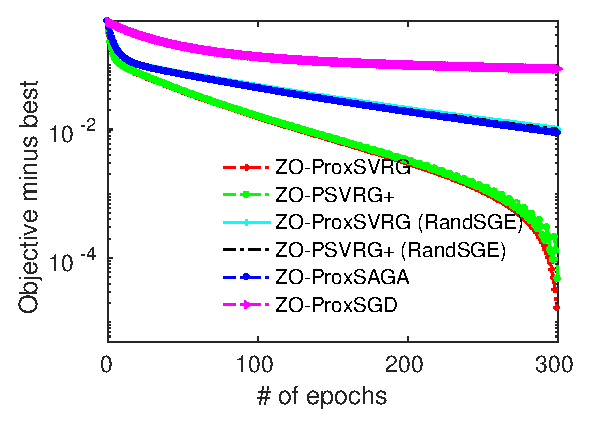
\includegraphics[width=0.24\linewidth]{Figures/binary/ijcnn1b50k1.eps}}%
\addtocounter{subfigure}{-4}
\subfigure{
\centering
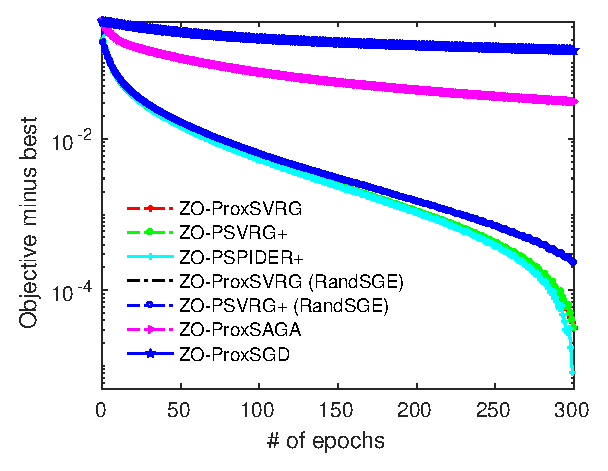
\includegraphics[width=0.24\linewidth]{Figures/binary/adultb50k1.eps}}%
%\subfigure{
%\centering
%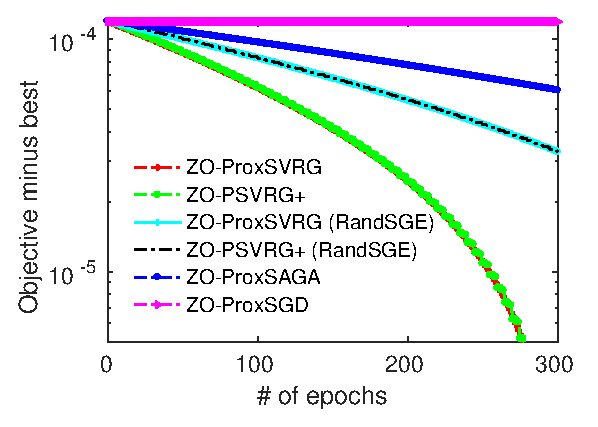
\includegraphics[width=0.24\linewidth]{Figures/binary/w8ab50k1.eps}}%
\subfigure{
\centering
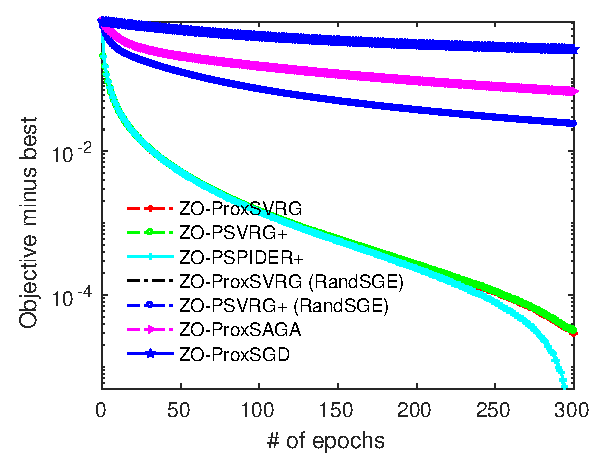
\includegraphics[width=0.24\linewidth]{Figures/binary/mnistb50k1.eps}}%
\end{figure*}
\begin{figure*}
\subfigure[comparison on ijcnn]{
\centering
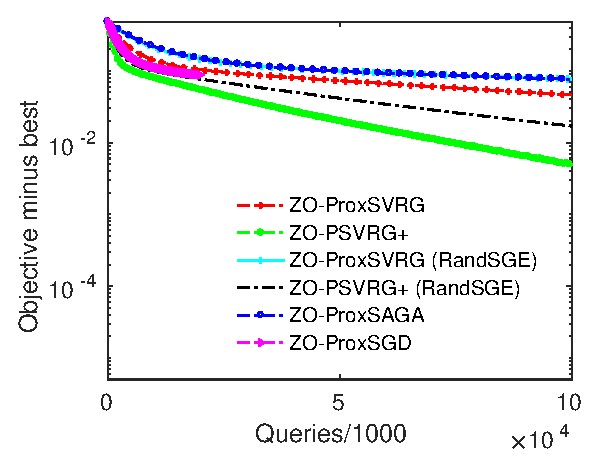
\includegraphics[width=0.24\linewidth]{Figures/binary/ijcnn1b50k2.eps}}%
\subfigure[comparison on covtype]{
\centering
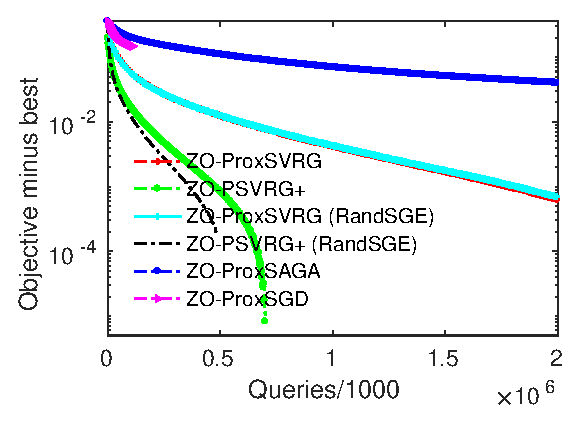
\includegraphics[width=0.24\linewidth]{Figures/binary/adultb50k2.eps}}%
\subfigure[comparison on real-sim]{
\centering
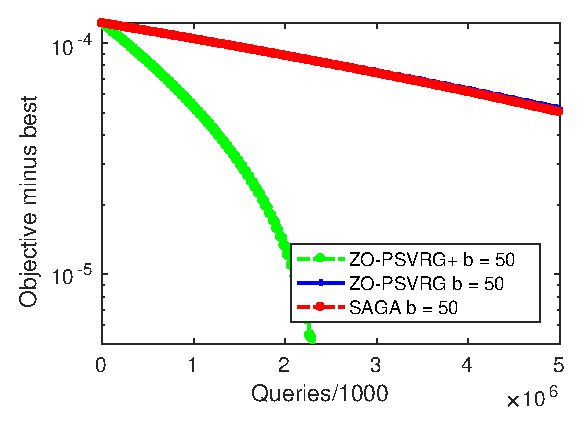
\includegraphics[width=0.24\linewidth]{Figures/binary/w8ab50k2.eps}}%
%\subfigure[comparison on rcv1]{
%\centering
%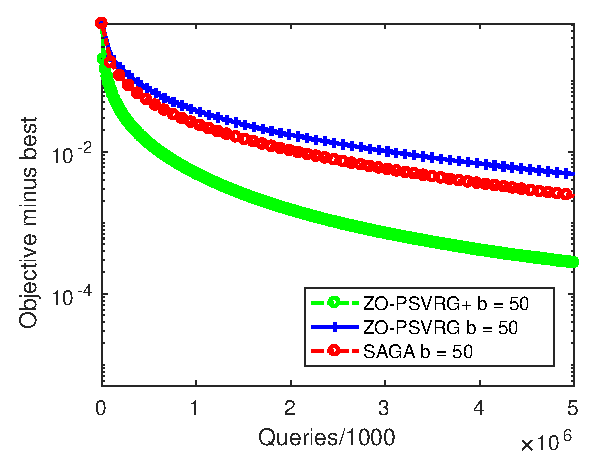
\includegraphics[width=0.3\linewidth]{Figures/binary/mnistb50k2.eps}}%
\setlength{\abovecaptionskip}{2pt}
\caption{Training loss residual $f(x) - f(x^*)$ versus iteration (top) and time (bottom) plot of Async-SVRG, ProxASAGA, Async-Katyusha, and Async-AcPSVRG. }
\label{fig:algo_comp}
\end{figure*}

\begin{figure*}[htbp]

\subfigure[comparison on ijcnn]{
\centering
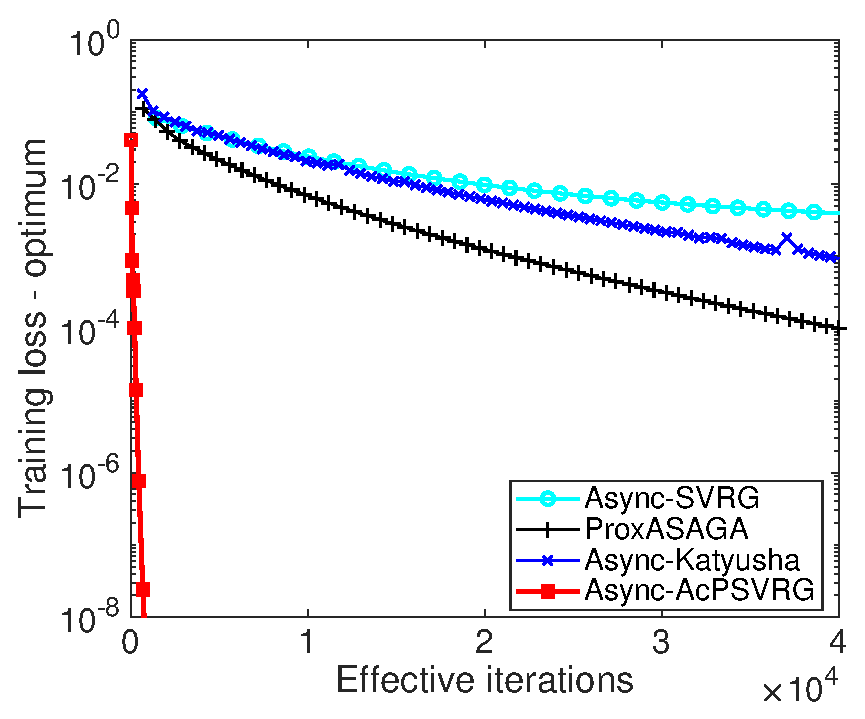
\includegraphics[width=0.24\linewidth]{Figures/ijcnn_obj_dev_comparison_16workers.eps}}%
\subfigure[comparison on covtype]{
\centering
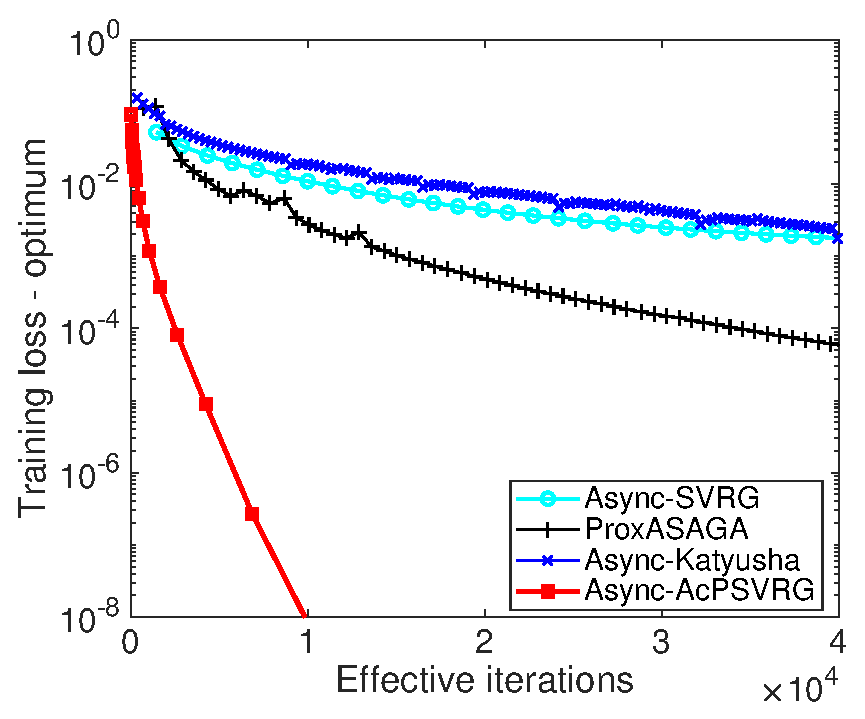
\includegraphics[width=0.24\linewidth]{Figures/covtype_obj_dev_comparison_16workers.eps}}%
\subfigure[comparison on real-sim]{
\centering
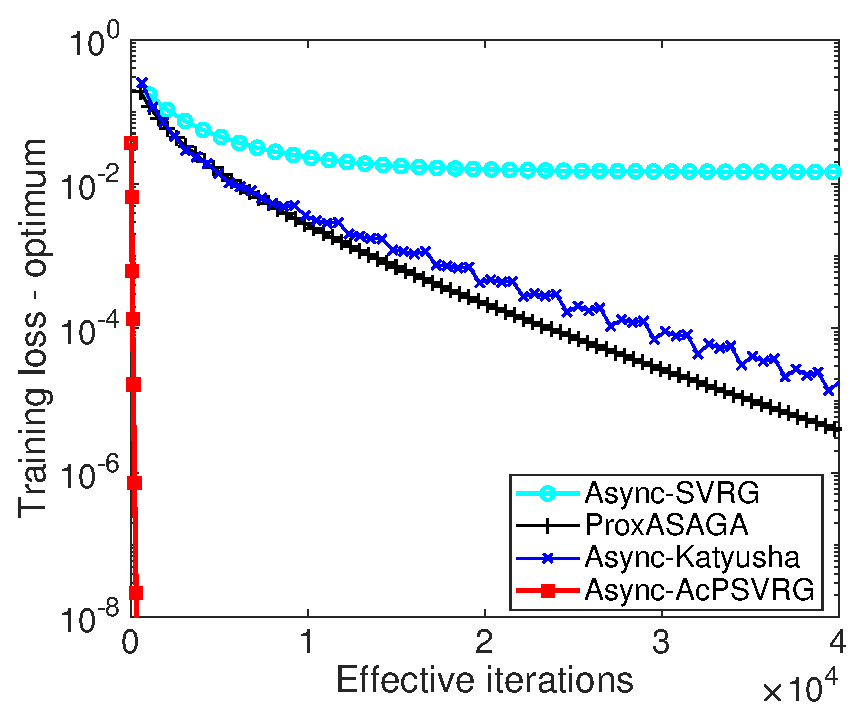
\includegraphics[width=0.24\linewidth]{Figures/real-sim_obj_dev_comparison_16workers.eps}}%
\subfigure[comparison on rcv1]{
\centering
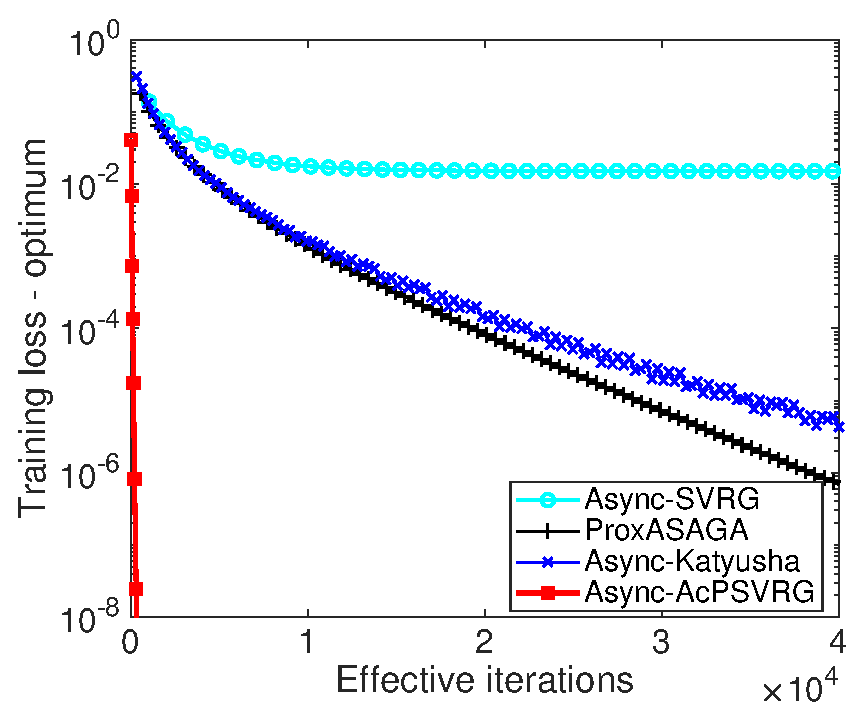
\includegraphics[width=0.24\linewidth]{Figures/rcv1_obj_dev_comparison_16workers.eps}}%

\subfigure[comparison on ijcnn]{
\centering
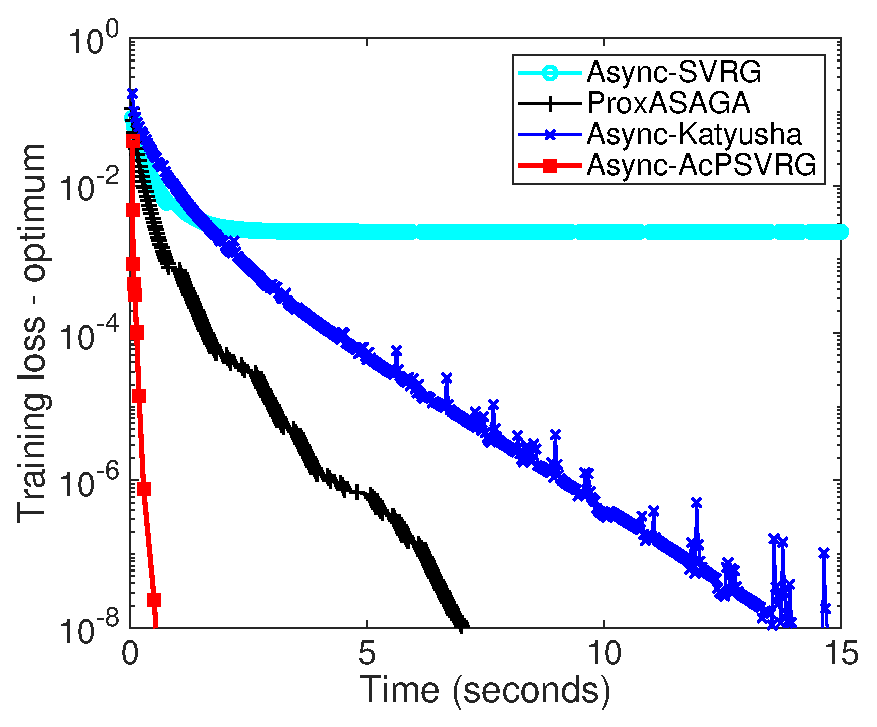
\includegraphics[width=0.24\linewidth]{Figures/ijcnn_obj_dev_comparison_time.eps}}%
\subfigure[comparison on covtype]{
\centering
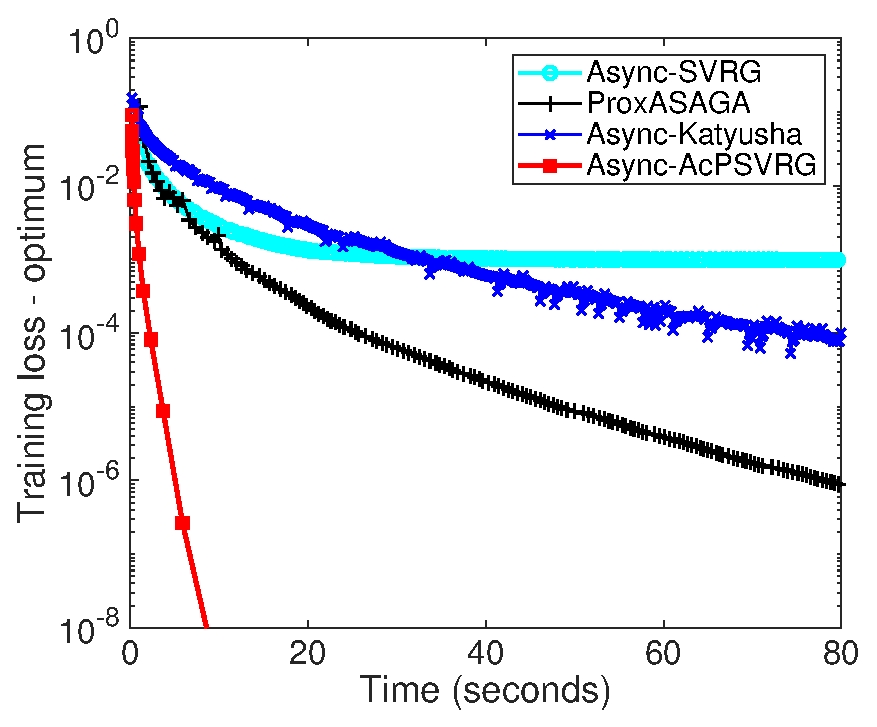
\includegraphics[width=0.24\linewidth]{Figures/covtype_obj_dev_comparison_time.eps}}%
\subfigure[comparison on real-sim]{
\centering
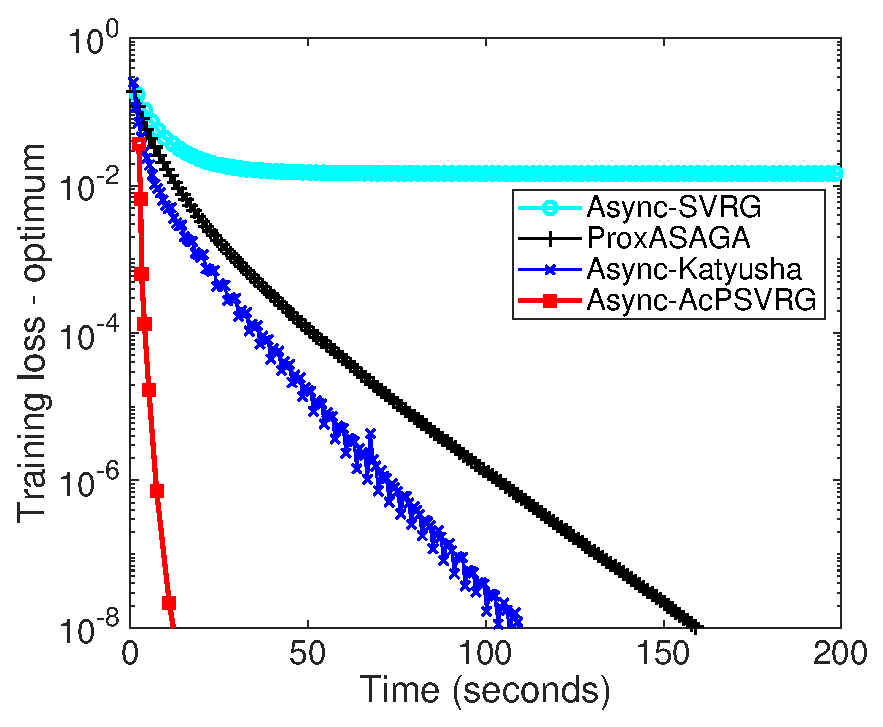
\includegraphics[width=0.24\linewidth]{Figures/real-sim_obj_dev_comparison_time.eps}}%
\subfigure[comparison on rcv1]{
\centering
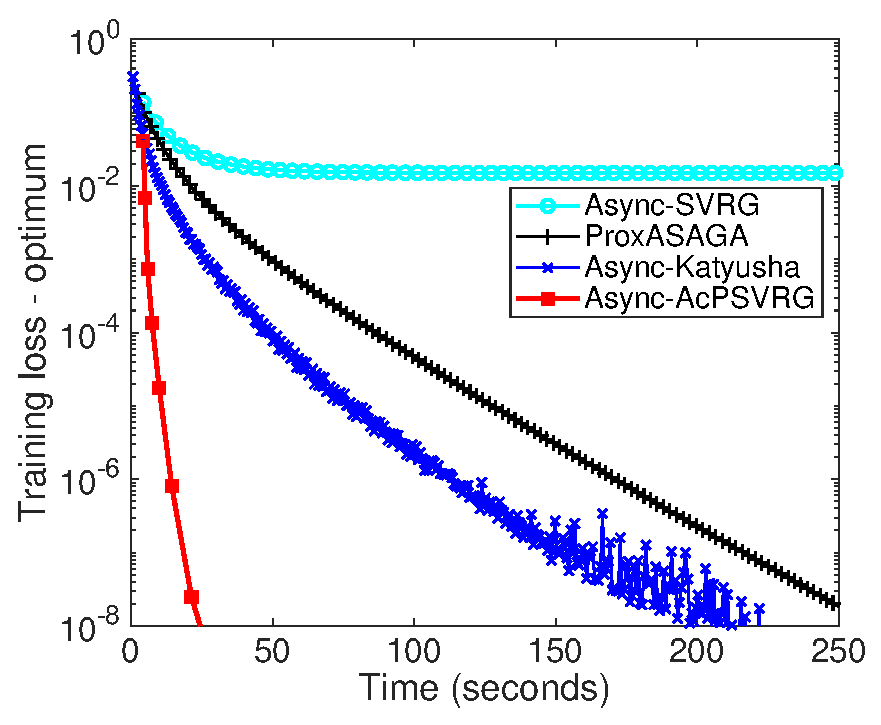
\includegraphics[width=0.24\linewidth]{Figures/rcv1_obj_dev_comparison_time.eps}}%
\setlength{\abovecaptionskip}{2pt}
\caption{Training loss residual $f(x) - f(x^*)$ versus iteration (top) and time (bottom) plot of Async-SVRG, ProxASAGA, Async-Katyusha, and Async-AcPSVRG. }
\label{fig:algo_comp}
\end{figure*}

  
\subsection{Adversarial Attacks on Black-Box DNNs}

{\color{Brown}
In image classification, adversarial
examples refer to carefully crafted perturbations such that, when added to the natural images, are
visually imperceptible but will lead the target model to misclassify. In the setting of "zeroth order"
attacks \cite{chen2017zoo,liu2018zeroth}, the model parameters are hidden and acquiring its gradient is inadmissible. Only
the model evaluations are accessible. We can then regard the task of generating a universal adversarial
perturbation (to $n$ natural images) as an ZO optimization problem of the form \eqref{problem}.
{\color{Green}
More exactly,
we use the zeroth-order algorithms to find a universal adversarial perturbation $x\in\R^d$ that could fool the samples $\{a_i \in \R^d, y_i\in\mathbb{N} \}_{i=1}^n$, which can be specified as the following elastic-net attacks to black-box DNNs problem:
\begin{equation}
\begin{split}
\min_{x\in\R^d} \frac{1}{n} \sum_{i=1}^n& \max\{F_{y_i}(a_i^{adv}) - \max_{j\neq y_i}F_j(a_i^{adv}),0\} + c\norm{a_i^{adv} - a_i}^2 \\
&+ \lambda_1 \norm{x}_{1} + \lambda_2 \norm{x}^{2}
\end{split}
\end{equation}
where $a_i^{adv} = 0.5\tanh(\tanh^{-1}(2a_i)+x)$ and $\lambda_1$ and $\lambda_2$ are nonnegative parameters to balance attack success rate, distortion and sparsity. Here $F(a) = \left[F_1(a),\ldots,F_K(a)\right]\in [0, 1]^K$ represents a well-trained DNN{\footnote{https://github.com/carlini/nn$\underline{~~}$robust$\underline{~~}$attacks}} for the MNIST handwritten digit classification, where $F_i(a)$ returns the prediction score of $i$-th class. {\color{Brown} The regularization parameter $c$ trades off adversarial success and the distortion of adversarial examples. In our experiment, we set the regularization parameter  $c = 0.2$. }

}

We choose $n = 10$ images from the same class, and set the same
parameters $b = 5$ and constant step size {\color{red} $30/d$} and {\color{red} $30/d$} for ZO-PSVRG+ (CoordSGE) and ZO-PSVRG+ (RandSGE), respectively, and $\eta = O(\frac{1}{d})$ with $\mu = O(\frac{1}{\sqrt{d}})$ for the competing algorithms, where $d = 28 \times 28$ is the image
dimension.


{\color{Green}
In addition, we set {\color{red} $\lambda_1 = 10^{-5}$} and {\color{red} $\lambda_2 = 10^{-5}$} in the experiment.
}
}
{\color{Melon}
Figure \ref{} and Figure \ref{} (in the supplementary materials) provide
comparison of the performance for the algorithms of interest.
Our two algorithms ZO-PSVRG+ (CoordSGE) and ZO-PSVRG+ (RandSGE) (with the large stepsize due to our improved analysis and $B < n$) have much better performance
both in convergence rate (iteration complexity) and
function query complexity than ZO-ProxSGD, ZO-ProxSVRG
and ZO-ProxSAGA. Our ZO-PSVRG+ (CoordSGE)
algorithm converges much faster than ZO-PSVRG+ (RandSGE)
in the initial optimization stage, and more importantly, has
much lower function query complexity, which is largely
due to the $O(\frac{1}{\sqrt{d}})$-level stepsize required by ZO-PSVRG+ (RandSGE).
}

{\color{Green}

Although having a relatively good performance in generating the adversarial samples, ZO-ProxSGD still shows worse performance than both the ZO-ProxSVRG and ZO-ProxSAGA, due to not using the VR technique.}
{\color{Brown}
Compared to ZO-ProxSGD, ZO-PSVRG+ offers a faster convergence due to $B < n$. In addition, ZO-PSVRG+ improves the $l_2$ distortion
of adversarial examples compared to ZO-ProxSGD (e.g., $30\%$ improvement when $q = 30$). 
}

\section{Appendix}
{\color{Green}
In this section, we provide the detailed proofs of the above lemmas and theorems. First, we give some useful properties of the CooSGE and the GauSGE, respectively.
}
\begin{lemma}[Three-Point Property] Let $F(\cdot)$ be a convex function, and let $D_{l}(\cdot,\cdot)$ be the Bregman distance for $l(\cdot)$. For a given vector $z$, let 
\[
z^+ = \text{arg}\,\,\min_{x\in\R^d}\{F(x)+D_{l}(x,z)\}.
\]
Then 
\begin{equation}
F(x) + D_l(x,z) \geq F(z^+) + D_l(x^+,z) + D_l(x,z^+)\qquad for\,\,all\,\,x\in\R^n
\end{equation}
with equality holding in the case when $F(\cdot)$ is a linear function and $l(\cdot)$ is a quadratic function.
\end{lemma}


\begin{lemma}\label{CooSGE}
Assume that the function $f(x)$ is $L$-smooth. Let $\hat{\nabla} f(x)$ denote the estimated gradient defined by CoordSGE. Define $f_{\mu_j} = \E_{u\sim U[\mu_j, \mu_j]} f(x+ue_j)$, where $U[-\mu_j,\mu_j]$ denotes the uniform distribution at the interval $[\mu_j, \mu_j]$. Then we have 
1) $f_{\mu_j}$ is $L$-smooth, and 
\begin{equation}
\hat{\nabla} f(x) = \sum_{j=1}^d \frac{\partial f_{\mu_j}}{\partial x_j}e_j
\end{equation} 
where $\partial f/\partial x_j$ denotes the partial derivative with respect to $j$th coordinate.

2) For $j\in [d]$, 
\begin{align}
\abs{f_{\mu_j}(x) - f(x)} &\leq \frac{L\mu_j^2}{2}\\
\abs{\frac{\partial f_{\mu_j}(x)}{\partial x_j}} \leq \frac{L\mu_j^2}{2}
\end{align}
 
 3) If $\mu = \mu_j$ for $j\in [d]$, then 
 \begin{equation}
 \norm{\hat{\nabla} f(x) - {\nabla} f(x)} ^2 \leq \frac{L^2 d^2 \mu^2}{4}
\end{equation}  
\end{lemma}

{\color{Sepia}
\begin{theorem}\label{SGERand-approx}
Assume that the function $f(x)$ is $L$-smooth. $\hat{\nabla}_r f(x)$ denote the estimated gradient defined by RandSGE. Define $f_{\mu} = \E_{u\sim N(0, I)}[f(x+\mu u)]$. Then, we have 

1) For any $x \in \R^d$, $\nabla f_{\mu}(x) = \E_u[\hat{\nabla}_r f(x,u)]$.\\
2) $\abs{f_{\mu}(x) - f(x)} \leq \frac{\mu^2 L}{2}$ and 
$\norm{f_{\mu}(x) - f(x)} \leq \frac{\mu L d}{2}$ for any $x \in \R^d$.\\
3) $\E_{u}\norm{\hat{\nabla}_r f(x,u) - \hat{\nabla}_r f(y,u)}^2 \leq 3dL^2\norm{x-y}^2 + \frac{3L^2d^2\mu^2}{2}$
\end{theorem}
}

\begin{lemma}\label{lemma1}
Let $x^+ = \Po_{\eta h}(x-\eta v)$, then the following inequality holds:
\begin{equation}\label{eq10}
F(x^+) \leq F(z) + \Iprod{\nabla f(x)-v}{x^+-z}-\frac{1}{\eta} \Iprod{x^+-x}{x^+-z}+\frac{L}{2}\norm{x^+-x}^2+\frac{L}{2}\norm{z-x}^2, \forall z\in \R^d. 
\end{equation}
\end{lemma}
\begin{proof}
First, we recall the proximal operator 
\begin{equation}\label{eq11}
\Po_{\eta h}(x-\eta v) := \text{arg}\,\,\min_{y\in\R^d}\left(h(y)+\frac{1}{2\eta}\norm{y-x}^2+\Iprod{v}{y}\right)
\end{equation}
For the nonsmooth function $h(x)$, we have 
\begin{equation}\label{eq12}
\begin{split}
h(x^+) &\leq h(z) + \Iprod{p}{x^+-z}\\
&= h(z) - \Iprod{v+\frac{1}{\eta}(x^+-x)}{x^+-z}
\end{split}
\end{equation}
where $p\in \partial h(x^+)$ such that $p+\frac{1}{\eta}(x^+-x)+v = 0$ according to the optimality condition of \eqref{eq11}, and \eqref{eq12} due to the convexity of $h$.
\begin{equation}\label{eq14}
f(x^+) \leq f(x)+\Iprod{\nabla f(x)}{x^+-x}+\frac{L}{2}\norm{x^+-x}^2
\end{equation}
\begin{equation}\label{eq15}
-f(z) \leq -f(x)+\Iprod{-\nabla f(x)}{z-x}+\frac{L}{2}\norm{z-x}^2
\end{equation}
where \eqref{eq14} holds since $f(x)$ has $L$-Lipschitz continuous gradient, and \eqref{eq15} holds since $-f(x)$ has the same $L$-Lipschitz continuous gradient as $f(x)$. 

 This lemma is proved by adding \eqref{eq12}, \eqref{eq14}, \eqref{eq15}, and recalling $F(x) = f(x)+h(x)$. 
\end{proof}
\begin{lemma}\label{lemm-est-grad}
Let  $x_{t}^s= \Po_{\eta h}(x_{t-1}^s - \eta \hat{v}_{t-1}^s)$ and $\overline{x}_{t}^s= \Po_{\eta h}(x_{t-1}^s - \eta \nabla f(x_{t-1}^s))$. Then the following inequality holds
\[
\Iprod{\nabla f(x_{t-1}^s) -\hat{v}_{t-1}^s)}{x_t^s -\overline{x}_t^s} \leq \eta\norm{\nabla f(x_{t-1}^s)-\hat{v}_{t-1}^s}^2
\]
\end{lemma}
\begin{proof}
First, we obtain $\norm{x_{t}^s-\overline{x}_{t}^s}$ and $\norm{\nabla f(x_{t-1}^s)-\hat{v}_{t-1}^s}$ as follows 
\begin{align}
h(x_t^s)&\leq h(\overline{x}_t^s) - \Iprod{\hat{v}_{t-1}^s+\frac{1}{\eta}(x_t^s-x_{t-1}^s)}{x_t^s-\overline{x}_t^s}\label{lemm-est-grad-1}\\
h(\overline{x}_t^s)&\leq h({x}_t^s) - \Iprod{\nabla f(x_{t-1}^s)+\frac{1}{\eta}(\overline{x}_t^s-x_{t-1}^s)}{\overline{x}_t^s-x_t^s}\label{lemm-est-grad-2}
\end{align}
where \eqref{lemm-est-grad-1} and \eqref{lemm-est-grad-2} hold due to \eqref{eq12}. Adding \eqref{lemm-est-grad-1} and \eqref{lemm-est-grad-2}, we have 
\begin{align}
\frac{1}{\eta}\Iprod{x_t^s -\overline{x}_t^s}{x_t^s -\overline{x}_t^s} &\leq \Iprod{\nabla f(x_{t-1}^s) -\hat{v}_{t-1}^s}{x_t^s -\overline{x}_t^s}\notag\\
\frac{1}{\eta}\norm{x_t^s -\overline{x}_t^s}^2 &\leq \norm{\nabla f(x_{t-1}^s) -\hat{v}_{t-1}^s}\norm{x_t^s -\overline{x}_t^s}\label{lemm-est-grad-3}\\
\norm{x_t^s -\overline{x}_t^s} &\leq \eta\norm{\nabla f(x_{t-1}^s) -\hat{v}_{t-1}^s}\label{lemm-est-grad-4}
\end{align}
where \eqref{lemm-est-grad-3} uses Cauchy-Schwarz inequality. Now this lemma is proved using Cauchy-Schwarz inequality and \eqref{lemm-est-grad-4}, i.e., $\Iprod{\nabla f(x_{t-1}^s) -\hat{v}_{t-1}^s)}{x_t^s -\overline{x}_t^s} \leq \norm{\nabla f(x_{t-1}^s)-\hat{v}_{t-1}^s} \norm{x_t^s -\overline{x}_t^s} \leq \eta\norm{\nabla f(x_{t-1}^s)-\hat{v}_{t-1}^s}^2$.
\end{proof}


\bibliographystyle{plainnat}
\bibliography{GTA}
\end{document}


